% SZTE Alkalmazott matematikus MSc záróvizsgatételek
%
% Szerzők:		Judák Regina
%				reginajudak@gmail.com
%
%				Majernyik Noel
%				majnol@vipmail.hu
%
%				Mezőfi Dávid
%				david.mezofi93@gmail.com
%
%%%%%%%%%%%%%%%%%%%%%%%%%%%%%%%%%%%%%%%%%%%%%%%%%%%%%%%%%%%%%%%%%%%%%%%%%%%%%%%%%%%%%%%%%%%%%%%%%%%%
%
% Creative Commons licenc
%
% Ez az alkotás a Creative Commons Nevezd meg! - Ne add el! - Így add tovább! 4.0 Nemzetközi licenc
% alá tartozik. A licenc megtekintéséhez látogass el a
% http://creativecommons.org/licenses/by-nc-sa/4.0/ oldalra.
%
%%%%%%%%%%%%%%%%%%%%%%%%%%%%%%%%%%%%%%%%%%%%%%%%%%%%%%%%%%%%%%%%%%%%%%%%%%%%%%%%%%%%%%%%%%%%%%%%%%%%
%
% PREAMBULUM
%
%%%%%%%%%%%%%%%%%%%%%%%%%%%%%%%%%%%%%%%%%%%%%%%%%%%%%%%%%%%%%%%%%%%%%%%%%%%%%%%%%%%%%%%%%%%%%%%%%%%%
%
% DIV=15 opcióval nem lesznek nagy margók, `twoside` opció a kétoldalas szedéshez.
\documentclass[DIV=15,appendixprefix]{scrreprt}
%
% Színes hivatkozásokhoz kommenteld ki az alábbi sort!
% Élő hivatkozások, indexek, PDF-ben, színesekhez: `colorlinks=true`
\usepackage[unicode,pdfborder={0 0 0},colorlinks=true]{hyperref}
%
%%%%%%%%%%%%%%%%%%%%%%%%%%%%%%%%%%%%%%%%%%%%%%%%%%%%%%%%%%%%%%%%%%%%%%%%%%%%%%%%%%%%%%%%%%%%%%%%%%%%
%
% Karakterkódolás és `babel` beállítása.
\usepackage[T1]{fontenc}
\usepackage[utf8]{inputenc}
% A `defaults=hu-min` opció biztosítja, hogy a tizedesvessző tizedesvessző legyen.
\def\magyarOptions{%
	defaults=hu-min}
\usepackage[magyar]{babel}
%
% A `description` környzetek "szépen" jelenjenek meg.
\def\descriptionlabel#1{\hskip\labelsep\normalfont\sffamily\bfseries #1.}
%%%%%%%%%%%%%%%%%%%%%%%%%%%%%%%%%%%%%%%%%%%%%%%%%%%%%%%%%%%%%%%%%%%%%%%%%%%%%%%%%%%%%%%%%%%%%%%%%%%%
%
% Tételszerű bekezdések.
\usepackage{amsthm}
\usepackage{amsmath, amssymb}
%
% Tétel és társai: félkövér + dőlt
\newtheorem*{tetel}{Tétel}
\newtheorem*{allit}{állítás}
\newtheorem*{kovet}{Következmény}
%
% Definíció és társai: félkövér + álló
\theoremstyle{definition}
\newtheorem*{defin}{Definíció}
\newtheorem*{feladat}{Feladat}
%
% Megjegyzés és társai: dőlt + álló
\theoremstyle{remark}
\newtheorem*{megj}{Megjegyzés}
\newtheorem*{utmut}{Útmutatás}
\newtheorem*{pelda}{Példa}
%
%%%%%%%%%%%%%%%%%%%%%%%%%%%%%%%%%%%%%%%%%%%%%%%%%%%%%%%%%%%%%%%%%%%%%%%%%%%%%%%%%%%%%%%%%%%%%%%%%%%%
%
% Számozások
%
% A feladat környzet számozása 17-tel kezdődik.
%\addtocounter{feladat}{16}
%
% Az egyenletek számozása szakaszokkal együtt történjen.
%\numberwithin{equation}{section}
%
%%%%%%%%%%%%%%%%%%%%%%%%%%%%%%%%%%%%%%%%%%%%%%%%%%%%%%%%%%%%%%%%%%%%%%%%%%%%%%%%%%%%%%%%%%%%%%%%%%%%
%
% Szépen szedett algoritmusok.
%
\usepackage[ruled,section]{algorithm}
\usepackage[noend]{algpseudocode}
\algrenewcommand\algorithmicrequire{\textbf{Bemenet}:}
\algrenewcommand\algorithmicensure{\textbf{Kimenet}:}
\newcommand{\Break}{\State\textbf{break} }
%
\usepackage{caption}
\makeatletter
\renewcommand{\ALG@name}{algoritmus}
\makeatother
\makeatletter
\DeclareCaptionLabelFormat{hunalg}{#2.~\ALG@name.}
\makeatother
\captionsetup[algorithm]{labelformat=hunalg}
% Példa.
%
%\begin{algorithm}
%	\caption{Cím}
%	\begin{algorithmic}
%		\Procedure{Kiír}{}
%			\While{$\diamond$ utáni bináris szám nem 0}
%				\State Kiírjuk a munkaszalag $\diamond$-ig lévő tartalmát, $a^{n}$-t.%
%					\Comment{Folytatólagosan írunk.}
%				\State Csökkentjük 1-gyel a $\diamond$ utáni bináris számot.%
%					\Comment{Vonjunk ki belőle 1-et.}
%			\EndWhile
%		\EndProcedure
%	\end{algorithmic}
%\end{algorithm}
%
%%%%%%%%%%%%%%%%%%%%%%%%%%%%%%%%%%%%%%%%%%%%%%%%%%%%%%%%%%%%%%%%%%%%%%%%%%%%%%%%%%%%%%%%%%%%%%%%%%%%
%
% Egyebek
%
% Grafikai csomagok betöltése.
\usepackage{graphicx}
%\usepackage{eso-pic}
%
% A képek elérési útvonalának megadása.
%\graphicspath{{./figures/}}
% Nyomdai minőségű táblázatok készítéséhez a `booktabs` csomag szükséges.
%\usepackage{booktabs}
%
% "Dummy" szöveg: Lipsum dolor sit amet...
\usepackage{lipsum}
%
% Szövegközi "ferdetört". Használat: `\sfrac{num}{den}`.
%\usepackage{xfrac}
%
% Az `enumitem` csomag színes-szagos `enumerate` környezetet biztosít.
\usepackage{enumitem}
\setlist[description]{labelindent=\parindent}
% Példa a használatra:
%
%\begin{enumerate}[label = (H-\arabic{*}), ref = H-\arabic{*}, leftmargin = *,%
%		 labelindent = \parindent, mode = unboxed]
%	\item
%\end{enumerate}
%
% Az írógép típusú betűtípus legyen Inconsolata.
% Másik hasznos a `courier`: ha dőlt, félkövér és egyebek is kellenek.
%\usepackage{inconsolata}
%
% Többsoros kommentek `verbatim` környezettel.
%\usepackage{verbatim}
%
% A következő csomag feltételezi, hogy van működő SAGE telepítve a SageTex csomaggal együtt.
%\usepackage{sagetex}
%
% Kontinentális mondatközök.
\frenchspacing
%
% Fejezetcímek magyar formátumnak megfelelően.
\renewcommand*{\chapterformat}{\thechapter\autodot\ \chapappifchapterprefix\enskip}
%
% Minden szakasz új oldalon kezdődjön.
%\usepackage{titlesec}
%\newcommand{\sectionbreak}{\clearpage}
%
%%%%%%%%%%%%%%%%%%%%%%%%%%%%%%%%%%%%%%%%%%%%%%%%%%%%%%%%%%%%%%%%%%%%%%%%%%%%%%%%%%%%%%%%%%%%%%%%%%%%
%
% Saját matematikai parancsok:
\newcommand{\ball}{\mathbb{B}}
\newcommand{\sphere}{\mathbb{S}}
\newcommand{\mean}{\mathbb{E}}
\newcommand{\prob}{\mathbb{P}}
\newcommand{\sd}{\mathbb{D}}
\newcommand{\BinomialD}{\mathcal{B}}
\newcommand{\imag}{\mathfrak{i}}
\newcommand{\SAGE}{\textsf{\textbf{SAGE}}{}}
\newcommand{\normald}{\mathcal{N}}
\newcommand{\wishartd}{\mathcal{W}}
\renewcommand{\tan}{\mathop{\mathrm{tg}}}
\DeclareMathOperator{\conv}{conv}
\DeclareMathOperator{\interior}{int}
\newcommand{\ballin}{\interior\mathbb{B}}
\DeclareMathOperator{\relint}{relint}
\DeclareMathOperator{\cl}{cl}
\DeclareMathOperator{\T}{T}
\DeclareMathOperator{\supp}{supp}
\DeclareMathOperator{\dom}{dom}
\DeclareMathOperator{\diag}{diag}
\DeclareMathOperator{\SO}{SO}
\DeclareMathOperator{\lnko}{lnko}
\DeclareMathOperator{\ind}{ind}
%
%%%%%%%%%%%%%%%%%%%%%%%%%%%%%%%%%%%%%%%%%%%%%%%%%%%%%%%%%%%%%%%%%%%%%%%%%%%%%%%%%%%%%%%%%%%%%%%%%%%%
% Irodalomjegyzék beállításai
\makeatletter
\let\old@thebibliography\thebibliography
\def\thebibliography#1{
\old@thebibliography{#1}
\@ifundefined{chapter}
{\addcontentsline{toc}{section}{\refname}}
{\addcontentsline{toc}{chapter}{\bibname}}}
\makeatother
%
%%%%%%%%%%%%%%%%%%%%%%%%%%%%%%%%%%%%%%%%%%%%%%%%%%%%%%%%%%%%%%%%%%%%%%%%%%%%%%%%%%%%%%%%%%%%%%%%%%%%
%
% Cím és társai
%
\titlehead{Szegedi Tudományegyetem\\%
	Természettudományi és Informatikai Kar\\%
	Bolyai Intézet}
\subject{Alkalmazott matematikus MSc}
\title{Záróvizsgatételek}
\subtitle{Általános szakirány}
\author{Judák Regina\\\texttt{reginajudak@gmail.com}%
	\and%
	Majernyik Noel\\\texttt{majnol@vipmail.hu}
	\and%
	Mezőfi Dávid\\\texttt{david.mezofi93@gmail.com}}
\date{Utoljára módosítva: \today}
%\publishers{asd}
%%%%%%%%%%%%%%%%%%%%%%%%%%%%%%%%%%%%%%%%%%%%%%%%%%%%%%%%%%%%%%%%%%%%%%%%%%%%%%%%%%%%%%%%%%%%%%%%%%%%
%
% DOKUMENTUM
%
%%%%%%%%%%%%%%%%%%%%%%%%%%%%%%%%%%%%%%%%%%%%%%%%%%%%%%%%%%%%%%%%%%%%%%%%%%%%%%%%%%%%%%%%%%%%%%%%%%%%
%
\begin{document}
%
% Cím
\maketitle
%
% Licenc
\minisec{Creative Commons licenc}
\begin{center}
	\includegraphics{by-nc-sa.eps}
\end{center}
Ez az alkotás a \emph{Creative Commons Nevezd meg! -- Ne add el! -- Így add tovább! 4.0 Nemzetközi
licenc} alá tartozik. A licenc megtekintéséhez látogass el a
\url{http://creativecommons.org/licenses/by-nc-sa/4.0/} oldalra.
%
% Tartalomjegyzék
\tableofcontents
%
%%%%%%%%%%%%%%%%%%%%%%%%%%%%%%%%%%%%%%%%%%%%%%%%%%%%%%%%%%%%%%%%%%%%%%%%%%%%%%%%%%%%%%%%%%%%%%%%%%%%
%
% Mindkét szakirányon közös tételek
%
\chapter{Mindkét szakirányon közös tételek}
%
\section{Gráfelmélet: összefüggőség, színezések}
%
\section{Gráfelmélet: párosítások, síkgráfok}
%
\section{Gröbner-bázisok és alkalmazásaik}
A tételhez kapcsolódó anyagrészek megtalálhatóak \textsc{Skublics Benedek}: \emph{Algoritmuselmélet -- Jegyzet Zádori László előadásához} \cite{Zadori} című jegyzetében.
%
\section{Matematikai titkosírások}
A tételhez kapcsolódó anyagrészek megtalálhatóak \textsc{Skublics Benedek}: \emph{Algoritmuselmélet -- Jegyzet Zádori László előadásához} \cite{Zadori} című jegyzetében.
%
\minisec{Alapfogalmak és célok}
A \emph{kriptológia} a titkosírás tudománya, melynek két fő ága van.
\begin{description}
	\item[Kriptográfia] Titkosírási rendszerek \emph{tervezése}.
	\item[Kriptoanalízis] Titkosírási rendszerek \emph{megfejtése}.
\end{description}
\emph{A kriptográfia alapfeladata} annak a problémának a megoldása, hogy két pont között úgy tudjunk
titkos üzenetet küldeni, hogy a küldés során az üzenet mindvégig titkos maradjon. Erre az
\emph{alapeljárás} a következő: $ A $ és $ B $ szeretne titkos üzenetet váltani, mely üzenet legyen
$ x $. Ehhez szükségük van egy-egy titkos kulcsra, legyenek ezek: $ a $ és $ b $. Szükséges továbbá
egy $ E $ kódoló és egy $ D $ dekódoló függvény. $ A $ kódolt üzenete $ E \left( x,{} a \right) $,
melyet elküld $ B $-nek, aki dekódolja: $ D \left(  E \left( x,{} a \right),{} b \right) = x $, így
visszakapva az eredeti $ x $ üzenetet.
%
\minisec{Nyilvános kulcsú titkosírás}
Az alapfeladat megoldására több lehetőségünk is van, az egyik ilyen a \emph{nyilvános kulcsú
titkosírások}. A nyilvános kulcsú titkosírásokkal bizonyos feltételek mellett az is ellenőrizhető,
hogy az üzenetet ki küldte (hitelesítés, autentikáció).

Az alapelv a következő: adott felhasználók egy $ \left\{ F_{ 1 },{} F_{ 2 },{} \ldots,{} F_{ n }
\right\} $ halmaza, mindenkinek rendelkeznie kell egy $ k_{ i } $ nyilvános és egy $ l_{ i } $
titkos kulccsal. Egy $ f $ függvényt \emph{kódoló és dekódoló függvénynek} nevezünk, ha teljesülnek
az alábbiak:
	\begin{enumerate}
		\item $ f \left( f \left( x,{} k_{ i } \right), {} l_{ i } \right) = x $ minden $ x $
			üzenetre és indexre;
		\item $ x $ és $ y $ ismeretében $ f \left( x,{} y \right) $ gyorsan számolható;
		\item $ y $ és $ f \left( x,{} y \right) $ ismeretében $ x $ nem számolható gyorsan;
		\item\label{itm:felt} ha $ f \left( f \left( x,{} l_{ i } \right), {} k_{ i } \right) = x $
			is teljesül minden $x$ üzenetre és indexre, akkor hitelesíteni is tudjuk az üzenet
			küldőjét.
	\end{enumerate}
Ekkor az eljárás a következő: tegyük fel,hogy $ F_{ 1 } $ küld üzenetet $ F_{ 2 }$-nek. $ F_{ 1 } $
az $ f \left( x,{} k_{ 2 } \right) $-t küldi el $F_{ 2 } $-nek, aki ezután kiszámolja $ f \left( f
\left( x,{} k_{ 2 } \right), {} l_{ 2 } \right)=x $-et.

Ha \aref{itm:felt}.~feltétel is teljesül, akkor $ F_{ 1 } $ az $ f \left( f \left( x,{} l_{ 1 }
\right), {} k_{ 2 } \right) $-t küldi el $F_{ 2 } $-nek, aki az $ f \left( f \left( f \left( f
\left( x,{} l_{ 1 } \right), {} k_{ 2 } \right),{} l_{ 2 } \right),{} k_{ 1 } \right) $-et számolja
ki.
%
\minisec{RSA}
Minden $ F_{ i } $ felhasználó a következőeket teszi:
\begin{itemize}
	\item választ két nagy prímet: $ p_{ i },{} q_{ i }$;
	\item kiszámolja a szorzatuk: $ m_{ i } =  p_{ i } q_{ i } $;
	\item $ k_{ i } $ szám választása úgy, hogy $ 1 < k_{ i } < \varphi \left( m_{ i } \right) $ és
		$\lnko \left( k_{ i },{} \varphi \left( m_{ i } \right) \right) = 1 $;
	\item $ l_{ i } $ kiszámolása: $ 1 < l_{ i } < \varphi \left( m_{ i } \right) $ és $ k_{ i }
		l_{ i } \equiv 1 \mod{ \varphi \left( m_{ i } \right) }$;
	\item \emph{nyilvános kulcs}: $ \left( k_{ i },{} m_{ i } \right) $;
	\item \emph{titkos kulcs}: $ \left( l_{ i },{} m_{ i } \right) $.
\end{itemize}
Az $ f \left( x,{} \left( y,{} z \right) \right) $ kódolófüggvény az $ \left( x,{} \left( y,{} z
\right) \right) $ párhoz az $ x^{ y } $ legkisebb nemnegatív maradékát rendeli modulo $ z $
(feltesszük, hogy az $ x $ üzenetre teljesül: $ 0 \le x < \min_{ i } m_{ i } $).
%
\minisec{Prímtesztek}
A prímszámok fontos szerepet játszanak a titkosírás során, teht szükségünk van olyan eljárásokra,
melyekkel tesztelni tudjuk egy számról, hogy prím vagy összetett szám-e. A kis Fermat-tétel egy
szükséges feltételt ad arra, hogy egy szám prímszám-e, a feltétel azonban nem fordítható meg.

\begin{description}
	\item[Soloway\,--\,Strassen] A jegyzetben nem szerepel, algoritmuselmélet gyakorlaton volt róla
		szó.
		\begin{algorithmic}[1]
			\Require{$ n $ és $ k $ számok}
			\For{$ i \gets 1,{} i < k,{} i \gets i + 1 $}
				\State $ a \gets $ \Call{Random}{$ 0,{} n - 1 $}
				\State $ x \gets a^{ \frac{ n - 1 }{ 2 } } \mod{ n }$
				\State $y \gets \left( \frac{ a }{ n }  \right) \mod{n}$
				\If{$ x \neq y $}
					\State \Return \texttt{$ n $ nem prím}
				\EndIf
			\EndFor
			\State \Return \texttt{$ n $ valószínűleg prím}
		\end{algorithmic}
		Ha $ n $ prím, akkor az output \emph{mindig} \texttt{$ n $ valószínűleg prím} lesz, ha $ n $
		összetett, akkor az output $ 1 - 2^{ - k } $ valószínűséggel \texttt{$ n $ nem prím}. Az
		$ x $ és $ y $ értékeknek az \emph{Euler-lemma} értelmében kell egyenlőnek lenniük feltéve,
		hogy $ n $ prím. Az $ \left( \frac{ a }{ n } \right) $ érték a \emph{Jacobi-szimbólum}.

	\item[Miller\,--\,Rabin] A Miller\,--\,Rabin-prímteszt egy egyszerű számelméleti észrevételen
		alapuló nem-determinisztikus prímteszt. Elvégzésével csupán nagy valószínűséggel
		állíthatjuk, hogy  a tesztelt szám prímszám. A tesztelés determinisztikussá tehető az
		általánosított Riemann-hipotézis segítségével.
	\item[AKS] Ez az első determinisztikus polinomiális futási idejű prímteszt, 2002-ből való és
		három indiai matematikus nevéhez kötődik: \emph{Agraval}, \emph{Kayal} és \emph{Saxena}. A
		gyakorlatban inkább a Miller\,--\,Rabint alkamazzák (gyorsabb, bár futásideje elméletileg
		nem polinomiális).
\end{description}
%
\minisec{A diszkrét logaritmus és alkalmazásai}
\begin{defin}
	Legyen $G$ egy véges ciklikus csoport, $ g \in G $ egy generátorelem és $ a \in G $ egy
	tetszőleges elem. Ekkor az $ a $ elem $ g $ alapú \emph{indexe/diszkrét logaritmusa} az a
	legkisebb nem negatív egész $ k $ szám, amelyre $ a = g^{ k }$, jelölésben $ \ind_{ g } a $.
\end{defin}
A diszkrét logaritmus kiszámítására nem ismert hatékony algoritmus, még akkor sem, ha ciklikus
csoportok helyett csak a $ \mathbb{ Z }_{ p }^{ * } $ alakú csoportokra szorítkozunk. Ezt a
problémát használja ki a következő két algoritmus.
\begin{description}
	\item[Diffie\,--\,Hellman-kulcsváltás] Az eljárás a diszkrét logaritmus problémáján alapszik. Az
		eljárás célja, hogy két felhasználó számára egy közös titkos kulcsot hozzon létre nyilvános
		kommunikációs csatornán keresztül.

	\item[Massey\,--\,Omura-rejtjelrendszer] Ez az eljárás is a diszkrét logaritmus problémáján
		alapszik, segítségével a felek biztonságosan tudnak titkos üzenetet küldeni egymásnak.

		Dióhéjban: elküldök egy ládát lelakatolva $ B $-nek, ő is ráteszi a saját lakatját,
		és visszaküldi nekem, én leveszem a saját lakatomat, és visszaküldöm $ B $-nek, aki így
		már ki tudja nyitni a ládát.
\end{description}
%
\section{Többváltozós és vektorértékű függvények}
%
\section{Fourier-sorok, ortogonális polinomok, sorfejtések}
%
\section{Közönséges differenciálegyenletek és elsőrendű parciális differenciálegyenletek}
%
\section{Többdimenziós normális eloszlású vektorok statisztikai analízise}
A tételhez kapcsolódó anyagrészek megtalálhatóak a \textsc{Bolla Marianna\,--\,Krámli András}:
\emph{Statisztikai következtetések elmélete} \cite{BollaKramli} című könyvben.

\begin{defin}[$ p $-dimenziós standard normális eloszlás] Az $ \mathbf{ Y } $ véletlen vektor
	\emph{$ p $-dimenziós standard normális eloszlású} -- jelölésben $ \mathbf{ Y } \sim
	\normald_{ p } \left( \mathbf{ 0 },{} \mathbf{ I }_{ p } \right) $ --, ha komponensei
	egydimenziós standard normális eloszlásúak és függetlenek.
\end{defin}
Ha $ \det \mathbf{ A } \neq 0 $ és $ \mathbf{ X } = \mathbf{ A } \mathbf{ Y } + \mathbf{ m } $,
akkor $ \mathbf{ X } \sim \normald_{ p } \left( \mathbf{ m },{} \mathbf{ C } \right) $, ahol
$ \mathbf{ C } = \mathbf{ A } \mathbf{ A }^{ \T } $ ($ \mathbf{ C } $ szimmetrikus és pozitív
definit, mivel \emph{Gram-mátrix} és $ \mathbf{ A } $ nemszinguláris).
%
\minisec{Wishart-eloszlás}\leavevmode
\begin{description}
	\item[Wishart-mátrix] A $ p \times  p $-s $ \mathbf{ W } $ véletlen mátrixot
		\emph{$ p $-dimenziós, $ n $ szabadságfokú} $ \mathbf{ C } $ kovarianciamátrixú (centrális)
		\emph{Wishart-mátrixnak} nevezzük, ha előállítható $ \mathbf{ W } = \mathbf{ X }
		\mathbf{ X }^{ \T } $ alakban, ahol a $ p \times n $-es $ \mathbf{ X } $ véletlen mátrix
		oszlopvektorai függetlenek és $ \normald_{ p } \left( \mathbf{ 0 },{} \mathbf{ C } \right) $
		eloszlásúak.
	\item[Wishart-eloszlás] Ilyen mátrix elemeinek együttes eloszlását $ \left( p,{} n,{}
		\mathbf{ C } \right) $ paraméterű (centrális) \emph{Wi\-shart-eloszlásnak} nevezzük --
		jelölésben $ \mathbf{ W } \sim \wishartd_{ p } \left( n,{} \mathbf{ C } \right) $.
\end{description}
$ \mathbf{ W } $ szimmetriája miatt valójában $ \frac{ p
\left( p + 1 \right) }{ 2 } $-dimenziós eloszlásról van szó. \emph{Nem centrális} Wishart-eloszlás
esetén a kapcsolódó $ \mathbf{ X } $ mátrix oszlopvektroai $ \normald_{ p } \left( \mathbf{ m },{}
\mathbf{ C } \right) $ eloszlásúak. Az $ \mathbf{ X } $ mátrix oszlopvektorainak segítségével
$ \mathbf{ W } $ előállítható \emph{diádösszegként}. \emph{Standard Wishart-eloszlás}:
$ \wishartd_{ p } \left( n,{} \mathbf{ I } \right) $, a standard Wishart-eloszlás $ p  = 1 $ mellett
éppen a $ \chi^{ 2 } \left( n \right) $-eloszlás.

Egy Wishart-mátrix standardizáltja standard Wishart-eloszlású \cite[5. fejezet, 4. szakasz, 4.1.
tétel]{BollaKramli}. Azonos dimenziójú és kovarianciamátrixú Wishart-mátrixok összegének
szabadságfoka az összeadandók szabadságfokainak összege \cite[5. fejezet, 4. szakasz, 4.2.
állítás]{BollaKramli}. Nem elfajult $ p $-dimenziós normális eloszlású minta mintaátlagának $ \left(
\bar{ \mathbf{ X } } \right) $, valamint empirikus kovarianciamátrix $ n $-szeresének $ \left(
\mathbf{ S } \right) $ eloszlása \cite[5. fejezet, 4. szakasz, 4.3. tétel]{BollaKramli}.

Definíciója miatt a Wishart-mátrix szimmetrikus és pozitív szemidefinit ($ n > p $ esetén belátható,
hogy majdnem biztosan pozitív definit is).
%
\minisec{Paraméterbecslés}
Legyen $ \mathbf{ X }_{ 1 },{} \mathbf{ X }_{ 2 },{} \ldots,{} \mathbf{ X }_{ n } $ független elemű
minta az $ \mathbf{ X } \sim \normald_{ p } \left( \mathbf{ m },{} \mathbf{ C } \right) $ véletlen
vektorra, tegyük fel, hogy $ n > p $. A mintaelemek alapján szeretnénk becslést adni az ismeretlen
$ \mathbf{ m } $ várható érték vektorra és a $ \mathbf{ C } $ kovarianciamátrixra, melyről
feltesszük, hogy pozitív definit. Ehhez a \emph{maximum likelihood módszert használjuk}, azaz a
mintaelemek együttes sűrűségfüggvényével definiált likelihhod-függvényt maximalizáljuk a két
ismeretlen paraméterben.

A paraméterek ML-becslése a fenti feltevések mellett: $ \hat{ \mathbf{ m } } =
\bar{ \mathbf{ X } } $ és $ \hat{ \mathbf{ C } } = \frac{ 1 }{ n } \mathbf{ S } $ (lásd
\cite[5.~fejezet, 5.~szakasz, 5.1.~tétel]{BollaKramli}). Így már levezehető a (standard)
Wishart-mátrix sűrűségfüggvényének képlete \cite[5.~fejezet, 5.~szakasz, 5.2. és
5.3.~tétel]{BollaKramli}. Ebből levezethető a standard Wishart-mátrix sajátértékeinek együttes
sűrűsége \cite[5.~fejezet, 5.~szakasz, 5.4.~tétel]{BollaKramli}, megemlítendő, hogy véletlen
mátrixok sajátértékei fontos szerepet játszanak a kvantummechanikában (\textsc{Wigner Jenő}).
%
\minisec{Hipotézisvizsgálat}
Az egydimenziós esethez hasonlóan bevezethetjük a következő fogalmakat: torzítatlan, elégséges,
teljes statisztika. Belátható, hogy a fenti ML-becslés esetén $ \bar{ \mathbf{ X } } $ torzítatlan,
míg $ \frac{ 1 }{ n } \mathbf{ S } $ torzított, de $ \frac{ 1 }{ n - 1 } \mathbf{ S } $ már
torzítatlan becslés, mindkét becslés erősen konzisztens, az $ \left(  \bar{ \mathbf{ X } },{}
\frac{ 1 }{ n } \mathbf{ S } \right) $ pár elégséges statisztika, az $ \left(
\bar{ \mathbf{ X } },{} \frac{ 1 }{ n - 1 } \mathbf{ S } \right) $ pár pedig hatásos becslés
\cite[5. fejezet, 6. szakasz eleje]{BollaKramli}.
\begin{defin}[Hotelling-féle $ T^{ 2 } $-eloszlás]
	Legyen $ \mathbf{ X } \sim \normald_{ p } \left( \mathbf{ 0 },{} \mathbf{ I }_{ p } \right) $ és
	$ \mathbf{ W } \sim \wishartd_{ p } \left( n,{} \mathbf{ I }_{ p } \right) $ egymástól független
	véletlen vektor és véletlen mátrix. Ekkor a $ T^{ 2 } = n \mathbf{ X }^{ \T }
	\mathbf{ W }^{ - 1 } \mathbf{ X } $ valószínűségi változót \emph{Hotelling-féle
	$ T^{ 2 }$-eloszlásúnak} nevezzük $ n $ (szabadsági fok) és $ p $ paraméterekkel.
\end{defin}
A $ T^{ 2 } $-eloszlás a Student-féle $ t $-eloszlás többdimenziós általánosítása. Belátható, hogy
az $ \mathbf{ X } \sim \normald_{ p } \left( \mathbf{ m },{} \mathbf{ C } \right) $ és
$ \mathbf{ W } \sim \wishartd_{ p } \left( n,{} \mathbf{ C } \right) $ esetben $ T^{ 2 } = n \left(
\mathbf{ X } - \mathbf{ m } \right)^{ \T } \mathbf{ W }^{ - 1 } \left( \mathbf{ X } - \mathbf{ m }
\right) $ szintén $ T^{ 2 } $-eloszlású $ n $ és $ p $ paraméterekkel \cite[5.~fejezet, 6.~szakasz,
6.1.~állítás]{BollaKramli}. A Hotelling-féle $ T^{ 2 } $-eloszlás és a Fisher-féle $ F $-eloszlás
kapcsolatát \cite[5.~fejezet, 6.~szakasz, 6.2.~tétel]{BollaKramli} részletezi.

A következő teszteket \cite[5.~fejezet, 6.~szakasz, 230--234. o.]{BollaKramli} részletezi.
\begin{description}
	\item[Várható érték tesztelése ismert kovarianciamátrix esetén]\leavevmode
		\begin{description}
			\item[Egymintás eset] Az $ \mathbf{ X } \sim \normald_{ p } \left( \mathbf{ m },{}
				\mathbf{ C } \right) $ véletlen vektorra vegyünk egy $ n > p $ elemű független
				mintát. Teszteljük, hogy $ \mathbf{ m } = \mathbf{ m }_{ 0 } $ teljesül-e. Ha
				$ H_{ 0 } $ igaz, akkor
				\begin{equation*}
					U_{ 1 } = \left( \bar{ \mathbf{ X } } -
					\mathbf{ m }_{ 0 } \right)^{ \T } \left( \frac{ 1 }{ n } \mathbf{ C }
					\right)^{ - 1 } \left( \bar{ \mathbf{ X } } - \mathbf{ m }_{ 0 } \right) \sim
					\chi^{ 2 } \left( p \right),
				\end{equation*}
				ez alapján tudunk dönteni. Ez az egymintás
				$ u $-próba magasabb dimenziós megfelelője.
			\item[Kétmintás eset] Az $ \mathbf{ X } \sim \normald_{ p } \left( \mathbf{ m }_{ 1 },{}
				\mathbf{ C }_{ 1 } \right) $, $ \mathbf{ Y } \sim \normald_{ p } \left(
				\mathbf{ m }_{ 2 },{} \mathbf{ C }_{ 2 } \right) $ véletlen vektorokra vegyünk
				rendre egy-egy $ n,{} m > p $ elemű egymástól független mintát (maguk a mintaelemek
				is függetlenek egymástól). Teszteljük, hogy $ \mathbf{ m }_{ 1 } =
				\mathbf{ m }_{ 2 } $ teljesül-e. Az előzőhöz hasonló statisztikát vizsgálunk.
		\end{description}
	\item[Várható érték tesztelése ismeretlen kovarianciamátrix esetén]\leavevmode
		\begin{description}
			\item[Egymintás eset] Az előző egymintás esethez hasonló statisztikát vizsgálunk, csak
			itt
			\begin{equation*}
				T^{ 2 } = \left( n - 1 \right) \left( \bar{ \mathbf{ X } } -
				\mathbf{ m }_{ 0 } \right)^{ \T } \hat{ \mathbf{ C } }^{ - 1 } \left( \bar{
				\mathbf{ X } } - \mathbf{ m }_{ 0 } \right)
			\end{equation*}
			statisztika és a korábbi Hotelling- és Fisher-eloszlás kapcsolatát felhasználva döntünk.
			Ez az egymintás $ t $-próba általánosításának tekinthető.
			\item[Kétmintás eset] Hasonlóan, csak feltesszük, hogy a két minta azonos
			kovarianciamátrixú. Itt is a Hotelling- és Fisher-eloszlás kapcsolatát felhasználva
			döntünk. Ha nem tesszük fel, hogy a kovarianciamátrixok megegyeznek, akkor is létezik
			próba a Welch-próbához hasonlóan.
		\end{description}
\end{description}
%
\section{Lineáris regresszió}
%
\section{Kontingenciatáblák elemzése}
%
\section{Diszkrét idejű Markov-láncok}
A tételhez kapcsolódó anyagrészek megtalálhatóak a \textsc{Pap Gyula\,--\,Szűcs Gábor}:
\emph{Sztochasztikus folyamatok} \cite{PapSzucs} című jegyzetben.
%
\section{Folytonos idejű Markov-láncok}
%
\section{Sztochasztikus folyamatok alapfogalmai}
%
\section{Optimalizálási eljárások}
%
\minisec{Alapfeladat és speciális esetei}
Legyen $ c \colon \mathbb{ R }^{ n } \supseteq \dom c \rightarrow \mathbb{ R } $ a
\emph{célfüggvény}, ekkor az optimalizálás feladata a $ c $ célfüggvény minimalizálása előre
kiszabott feltételek mellett:
\begin{equation*}
	\begin{array}{rcl}
		\mathbf{ x }					&	\in			&	\mathcal{ F }\\
		\hline
		c \left( \mathbf{ x } \right)	&	\rightarrow	&	\min
	\end{array} \quad \left( \mathbf{ x } \in \dom c \right).
\end{equation*}
Explicit feltételek:
\begin{equation*}
	\begin{cases}
		f_{ i } \left( \mathbf{ x } \right) \le 0,	&	i \in \left[ k \right] = \left\{ 1,{} 2,{}
			\ldots,{} k \right\};\\
		g_{ j } \left( \mathbf{ x } \right) = 0,	&	j \in \left[ \ell \right],
	\end{cases} \quad \Rightarrow \quad \begin{cases}
		f \left( \mathbf{ x } \right) \preceq \mathbf{ 0 };	&\\
		g \left( \mathbf{ x } \right) = \mathbf{ 0 }.		&
	\end{cases}
\end{equation*}
A $ \mathcal{ D } $ \emph{értelmezési tartomány} a $ c $, az $ f_{ i } $ és a $ g_{ j } $ függvények
értelmezési tartományainak metszete. A \emph{lehetséges megoldások halmaza}: $ \mathcal{ L } =
\mathcal{ D } \cap \mathcal{ F } $. Az $ \left( \mathbf{ x }^{ * },{} p^{ * } \right) $ párt
\emph{optimális helynek}, illetve \emph{optimális értéknek} nevezzük, ha
\begin{equation*}
	c \left( \mathbf{ x }^{ * } \right) = p^{ * } = \inf_{ \mathbf{ x } \in \mathcal{ L } } c \left(
	\mathbf{ x } \right) \in \mathbb{ R } \cup \left\{ - \infty \right\} \cup \left\{ \infty
	\right\}.
\end{equation*}
Gyakran megelégszünk \emph{$ \epsilon $-közelítő} $ \left( p^{ * } + \epsilon \right) $, illetve
\emph{-approximáló} $ \left( \left( 1 + \epsilon \right) p^{ * },{} \left( 1 - \epsilon \right)
p^{ * } \right) $ megoldásokkal. A problémák átfogalmazhatók a feltételek ekvivalens átalakításával,
\emph{slack}-változók bevezetésével (egyenlőtlenség kiküszöbölésére), valamint a célfüggvény monoton
függvénybe történő helyettesítésével.
\begin{description}
	\item[Feltétel nélküli optimalizálás] Legkisebb négyzetek problémája: $ \left\| \mathbf{ c } -
		\mathbf{ A } \mathbf{ x } \right\|^{ 2 } \rightarrow \min $ (egyenes illesztése mért
		adatpontokra)
	\item[LP-feladatok] \begin{equation}\tag{LP}
			\begin{array}{rcl}
				\mathbf{ A } \mathbf{ x }			&	=			&	\mathbf{ b }\\
				\mathbf{ x }						&	\succeq		&	\mathbf{ 0 }\\
				\hline
				\mathbf{ c }^{ \T } \mathbf{ x }	&	\rightarrow	&	\min
			\end{array}, \qquad \begin{array}{rcl}
				\mathbf{ A } \mathbf{ x }			&	\preceq		&	\mathbf{ b }\\
				\hline
				\mathbf{ c }^{ \T } \mathbf{ x }	&	\rightarrow	&	\min
			\end{array}.
		\end{equation}
	\item[SDP-feladatok] \begin{equation}\tag{SDP}
			\begin{array}{rcl}
				\sum_{ i = 1 }^{ n } x_{ i } \mathbf{ A }_{ i }		&	\preceq	&	\mathbf{ B }\\
				\mathbf{ D } \mathbf{ x }							&	=	&	\mathbf{ e }\\
				\hline
				\mathbf{ c }^{ \T } \mathbf{ x }	&	\rightarrow	&	\min
			\end{array}; \qquad \underbrace{\begin{array}{rcll}
				\left\langle \mathbf{ A }_{ i },{} \mathbf{ X } \right\rangle	&	=	&
					b_{ i }			&	i \in \left[ k \right]\\
				\mathbf{ X }													&	\succeq	&
					\mathbf{ 0 }	&\\
				\hline
				\left\langle \mathbf{ C },{} \mathbf{ X } \right\rangle			&	\rightarrow	&
					\min			&
			\end{array}}_{\text{I. normálforma}}; \qquad \underbrace{\begin{array}{rcl}
				\sum_{ i = 1 }^{ n } x_{ i } \mathbf{ A }_{ i }		&	\preceq	&	\mathbf{ B }\\
				\hline
				\mathbf{ c }^{ \T } \mathbf{ x }	&	\rightarrow	&	\min
			\end{array}}_{\text{II. normálforma}},
		\end{equation}
		ahol az $ \mathbf{ A }_{ i },{} \mathbf{ B },{} \mathbf{ C },{} \mathbf{ X } $ mátrixok
		szimmetrikusak.
\end{description}
%
\minisec{Lagrange-módszer}
\begin{equation*}\tag{Lagrange-függvény}
	L \left( \mathbf{ x };{} \lambda,{} \mu \right) = c \left( \mathbf{ x } \right) + \lambda^{ \T }
	f \left( \mathbf{ x }	\right) + \mu^{ \T } g \left( \mathbf{ x }	\right).
\end{equation*}
Ha $ \mathbf{ x } \in \mathcal{ L } $ és $ \lambda \succeq \mathbf{ 0 } $, akkor $ c \left(
\mathbf{ x } \right) \ge L \left( \mathbf{ x };{} \lambda,{} \mu \right) $. Így
\begin{equation}\tag{duális célfüggény, duális feladat}
	\tilde{ c } \left( \lambda,{} \mu \right) = \inf_{ \mathbf{ x } \in \mathcal{ D } } L \left(
	\mathbf{ x };{} \lambda,{} \mu \right), \qquad \begin{array}{rcl}
		\lambda										&		\succeq	&	\mathbf{ 0 }\\
		\hline
		\tilde{ c } \left( \lambda,{} \mu \right)	&	\rightarrow	&	\max
	\end{array}.
\end{equation}
\begin{tetel}[gyengedualitás-tétel]
	Legyen a duális feladat optimális értéke $ d^{ * } $. Ekkor $ p^{ * } \ge d^{ * } $.
\end{tetel}
\begin{megj}
	Ha egyenlőség teljesül, akkor \emph{erős dualitás}. Ha $ p^{ * } - d^{ * } > 0 $, akkor
	\emph{pozitív dualitási hézag}.
\end{megj}
%
\minisec{Karush\,--\,Kuhn\,--\,Tucker-tétel}
Tegyük fel, hogy $ g_{ i } $-k affin, $ c,{} f_{ i } $-k konvex és differenciálható függvények. Erős dualitás pontosan akkor teljesül, ha létezik $ \hat{ \mathbf{ x } } $, $ \left( \hat{ \lambda }
,{} \hat{ \mu } \right) $, melyek teljesítik a következő feltételeket:
\begin{enumerate}[label = (KKT--\arabic{*}), ref = KKT--\arabic{*}, mode = unboxed,%
	labelindent = \parindent, leftmargin = *]
	\item\label{kkt1} $ \hat{ \mathbf{ x } } $ primál lehetséges megoldás;
	\item\label{kkt2} $ \left( \hat{ \lambda },{} \hat{ \mu } \right) $ duál lehetséges megoldás;
	\item\label{kkt3} $ \hat{ \mathbf{ x } } $, $ \left( \hat{ \lambda },{} \hat{ \mu } \right) $
	komplementárisan laza tulajdonságú, azaz
		\begin{itemize}
			\item ha $ f_{ i } \left( \hat{ \mathbf{ x } } \right) < 0 $, akkor
				$ \hat{ \lambda }_{ i } = 0 $;
			\item ha $ \hat{ \lambda }_{ i } > 0 $, akkor $ f_{ i } \left( \hat{ \mathbf{ x } }
				\right) = 0 $;
		\end{itemize}
	\item\label{kkt4} $ \nabla c \left( \hat{ \mathbf{ x } } \right) + \left( \hat{ \lambda }
		\right)^{ \T } \nabla f \left( \hat{ \mathbf{ x } } \right) + \left( \hat{ \mu }
		\right)^{ \T } \nabla g \left( \hat{ \mathbf{ x } } \right) = 0 $.
\end{enumerate}
Ha létezik ilyen $ \hat{ \mathbf{ x } } $, $ \left( \hat{ \lambda } ,{} \hat{ \mu } \right) $, akkor $ \hat{ \mathbf{ x } } $ primál, $ \left( \hat{ \lambda } ,{} \hat{ \mu } \right) $ duál optimumhely.
%
\minisec{Súlyozott párosítási probléma}
\begin{feladat}
	Legyen a $ G $ gráf, valamint a $ c \colon E \rightarrow \mathbb{ R }^{ + } $ \emph{élsúlyozás}
	adott. Keressünk maximális súlyú párosítást!
\end{feladat}
A $ c $ súlyfüggvényt azonosíthatjuk egy $ \mathbf{ c } \in \mathbb{ R }^{ E } $ vektorral. Legyen
$ \mathbf{ B } $ a $ G $ gráf \emph{pont-él illeszkedési mátrixa}. Így a feladat:
\begin{equation*}
	\underbrace{\begin{array}{rcl}
		\mathbf{ B } \mathbf{ x }			&	\preceq	&	\mathbf{ 1 }\\
		\mathbf{ 0 }						&	\preceq	&	\mathbf{ x }\\
		\mathbf{ x }						&	\in		&	\mathbb{ Z }^{ E }\\
		\hline
		\mathbf{ c }^{ \T } \mathbf{ x }	&	\rightarrow	&	\max
	\end{array}}_{\text{egész feltételű LP}} \qquad \leadsto \qquad \underbrace{\begin{array}{rcl}
		\mathbf{ B } \mathbf{ x }			&	\preceq	&	\mathbf{ 1 }\\
		\mathbf{ 0 }						&	\preceq	&	\mathbf{ x }\\
		\hline
		\mathbf{ c }^{ \T } \mathbf{ x }	&	\rightarrow	&	\max
	\end{array}}_{\text{LP-relaxáció}} \qquad \Leftrightarrow \qquad \begin{array}{rcl}
		\mathbf{ M } \mathbf{ x }			&	\preceq	&	\begin{bmatrix}
				\mathbf{ 1 }\\
				\mathbf{ 0 }
			\end{bmatrix}\\
		\hline
		\mathbf{ c }^{ \T } \mathbf{ x }	&	\rightarrow	&	\max
	\end{array} \quad \left( \mathbf{ M } = \begin{bmatrix}
		\mathbf{ B }\\
		- \mathbf{ I }_{ E }
	\end{bmatrix} \right) .
\end{equation*}
Ha $ G $ \emph{páros}, akkor $ \mathbf{ B } $ (és így $ \mathbf{ M } $ is) \emph{totálisan
unimoduláris} (bármely aldeterminánsa $ - 1 $, $ 0 $ vagy $ 1 $), és ekkor a relaxált feladat
ekvivalens az eredetivel.
%
\minisec{LP és SDP kombinatorikai alkalmazásai}\leavevmode
\begin{description}
	\item[Folyamprobléma és duálisa] Legyen $ \mathcal{ H } = \left( \vec{ G },{} s,{} t,{} c
		\right) $ hálózat: $ s,{} t $ rendre \emph{forrás}, \emph{nyelő}, $ c $
		\emph{kapacitásfüggény} $ \left( \mathbf{ c } \right) $. Legyen a \emph{folyamfüggvény} $ f
		\colon E \rightarrow \mathbb{ R } $, azonosíthatjuk $ \mathbf{ x } $-szel.
		Teljesüljenek a kapacitásfeltételek: $ \mathbf{ 0 } \preceq \mathbf{ x } \preceq
		\mathbf{ c } $, valamint a Kirchhoff-törvény (csúcsonként a ki- és a beáramló mennyiség
		azonos). A folyam \emph{értéke}: $ v $, a forrásnál a kiáramló és beáramló mennyiség
		különbsége (nyelőnél fordítva).

		Adjunk hozzá $ \vec{ G } $-hez egy $ e_{ + } = \overrightarrow{ t s } $ élt, melyen a
		(kiterjesztett) folyam $ v $-t vesz fel. Ekkor $ \vec{ G }_{ + } $ cirkuláció.  A feladat és
		duálisa:
		\begin{equation}\tag{MFMC}
			\begin{array}{rclcl}
				\mathbf{ 0 }							&	\preceq		&	\mathbf{ x }	&	\preceq	&	\mathbf{ c }\\
				\mathbf{ B }_{ + } \mathbf{ x }_{ + }	&	=			&	\mathbf{ 0 }	&			&	\\
				\hline
				v										&	\rightarrow	&	\max
			\end{array} \qquad \leadsto\qquad \begin{array}{rcl}
				\mathcal{ V }					&				& \text{egy $ s $-$ t $-vágás}\\
				\hline
				C \left( \mathcal{ V } \right)	&	\rightarrow	&	\min
			\end{array}.
		\end{equation}
	\item[Maximális vágás problémája és duálisa] Legyen $ G = \left( V,{} E \right) $ egyszerű gráf.
		Keressünk olyan $ \mathcal{ V } $ vágást, melyre $ \left| E \left( \mathcal{ V } \right)
		\right| $ maximális! A feladat duálisa SDP-feladat ($ \mathbf{ A } $ a szomszédsági mátrix,
		$ \mathbf{ x } \in \left\{ -1,{} 1 \right\}^{ V } $ a vágást kódolja):
		\begin{equation*}
			\begin{array}{rcl}
				\mathbf{ A } + \diag \mu 	&		\succeq	&	\mathbf{ 0 }\\
				\hline
				- \mathbf{ 1 }^{ \T } \mu	&	\rightarrow	&	\max
			\end{array}.
		\end{equation*}
%		Egy $ \mathcal{ V } $ vágás: $ \mathbf{ x } \in \left\{ -1,{} 1 \right\}^{ V } \subset
%		\mathbb{ R }^{ V } $, ahol a komponens $ - 1 $, ha a megfelelő csúcs a vágás egyik, $ 1 $,
%		ha a vágás másik oldalára esik. Legyen $ \mathbf{ A } $ a gráf szomszédsági mátrixa. Az
%		$ \mathbf{ x }^{ \T } \mathbf{ A } \mathbf{ x } $ kvadratikus alakban az $ e = \left\{ u,{}
%		v \right\} $ él hozzájárulása $ 2 x_{ u } x_{ v } $, $ x_{ u } x_{ v } = 1 $, ha $ e $-t
%		\textqq{nem vágtuk ketté}, $ - 1 $ különben. A feladat és duálisa:
%		\begin{equation*}
%	 		\begin{array}{rcl}
%				x_{ v }^{ 2 } 									&		=		& 1 \quad \left(
%				\forall \, v \in V \right)\\
%				\hline
%				\mathbf{ x }^{ \T } \mathbf{ A } \mathbf{ x }	&	\rightarrow	&	\min
%			\end{array} \qquad \leadsto \qquad \begin{array}{rcl}
%				\mathbf{ A } + \diag \mu 	&		\succeq	&	\mathbf{ 0 }\\
%				\hline
%				- \mathbf{ 1 }^{ \T } \mu	&	\rightarrow	&	\max
%			\end{array}.
%		\end{equation*}
	\item[Maximális független ponthalmaz felső becslése]  Legyen $ G = \left( V,{} E \right) $
		egyszerű gráf, legyen $ \mathbf{ A } $ a gráf szomszédsági mátrixa. Jelölje $ \mathbf{ J } $
		a csupa 1 mátrixot, legyen $ \bar{ \mathbf{ A } } = \mathbf{ J } - \mathbf{ A } $. Ekkor, ha
		$ F \subseteq V $ független ponthalmaz, akkor $ \left. \bar{ \mathbf{ A } }
		\right|_{ F \times F } = \mathbf{ J } $. Sajátvektor-sajátértékekre vonatkozó
		észrevételekből adódik, hogy $ \left| F \right| \le \lambda_{ \max } \left(
		\bar{ \mathbf{ A } } \right) $, és így $ \alpha \left( G \right)  \le \lambda_{ \max }
		\left( \bar{ \mathbf{ A } } \right) $.

		A kapcsolódó SDP-feladat:
%
%		Nevezzünk egy $ V \times V $-s szimmetrikus $ \mathbf{ M } $ mátrixot \emph{$ T_{ G }
%		$-tulajdonságúnak}, ha a főátlón és a \textqq{neméleknél} is 1-es szerepel. Ekkor az ilyen
%		tulajdonságú mátrixok maximális sajátérékeinek minimuma is alkalmas felső becslés $ \alpha
%		\left( G \right) $-re. Így, ha $ \mathbf{ S }_{ e } $ az $ e $ élnek megfelelő szomszédsági
%		mátrix, akkor az SDP-feladat:
		\begin{equation*}
	 		\begin{array}{rcl}
				\mathbf{ M } 									&		=		& \mathbf{ J } -
					\sum_{ e \in E } x_{ e } \mathbf{ S }_{ e }\\
				\mu \mathbf{ I }_{ V } - \mathbf{ M }			&		\succeq	& \mathbf{ 0 }\\
				\hline
				\mu	&	\rightarrow	&	\min.
			\end{array}
		\end{equation*}
		Ennek a feladatnak a optimumát a \emph{$ G $ gráf Lovász-féle $ \theta $-függvényének}
		nevezzük, és $ \alpha \left( G \right) \le \theta \left( G \right) $.

		\emph{Lovász-féle szendvicstétel}: $ \alpha \left( G \right) \le \theta \left( G \right) \le
		\bar{ \chi } \left( G \right) \left( = \chi \left( \bar{ G } \right) \right) $.
\end{description}
%
\minisec{Egészértékű programozás}
\begin{equation}\tag{IP és LP-relaxáltja}
	\begin{array}{rcl}
		\mathbf{ A } \mathbf{ x } 			&	\preceq		&	\mathbf{ b }\\
		\mathbf{ x } 						&	\in			&	\mathbb{ N }^{ n }\\
		\hline
		\mathbf{ c }^{ \T } \mathbf{ x }	&	\rightarrow	&	\min.
	\end{array} \qquad \leadsto \qquad \begin{array}{rcl}
		\mathbf{ A } \mathbf{ x } 			&	\preceq		&	\mathbf{ b }\\
		\hline
		\mathbf{ c }^{ \T } \mathbf{ x }	&	\rightarrow	&	\min.
	\end{array}
\end{equation}
\begin{description}
	\item[L-következtetés] Szokásos \textqq{levezetés} révén nyert új egyenlőtlenség.
	\item[I-következtetés] Ha $ \alpha_{ 1 } x_{ 1 } + \alpha_{ 2 } x_{ 2 } + \ldots +
		\alpha_{ n } x_{ n } \le \beta $ Az egyenlőtlenségek egy következménye
		(L-következtetés), akkor $ \left\lfloor \alpha_{ 1 } \right\rfloor x_{ 1 } +
		\left\lfloor \alpha_{ 2 } \right\rfloor x_{ 2 } + \ldots + \left\lfloor \alpha_{ n }
		\right\rfloor x_{ n } \le \left\lfloor \beta \right\rfloor $ egy \emph{I-köveztetés}. Az
		új egyenlőtlenségnek a feltételekhez történő hozzáadásával nem veszítünk lehetséges
		megoldást.
	\item[Algoritmus] L- és I-következtetések végrehajtását (valamilyen sámát követve, pl.
		Gomory-al\-go\-rit\-must) követően megoldjuk a kapcsolódó LP-relaxált feladatot, ha a kapott
		megoldás egész koordinátájú, akkor készen vagyunk, ha nem, akkor új L- és
		I-következtetéseket hajtunk végre, és így tovább\ldots
%		\leavevmode%
%		\begin{algorithmic}[1]
%			\Procedure{Relaxáció}{IP-feladat}
%				\State Oldjuk meg az IP-feladat LP-relaxáltját!
%				\State\Return az LP-relaxált feladat optimumhelye
%			\EndProcedure
%			\Procedure{GoodLuck}{optimumhely}
%				\If{optimumhely egész koordinátájú}
%					\State\Return \textsc{true}
%					\Else
%						\State\Return \textsc{false}
%				\EndIf
%			\EndProcedure
%			\Procedure{MegoldIP}{IP-feladat}
%				\State optimumhely $\gets$ \Call{Relaxáció}{IP-feladat}
%				\If{\Call{GoodLuck}{optimumhely}}
%					\State\Return optimumhely
%					\Else
%					\State új IP-feladat $\gets$ L- és I-következtetések\Comment{Gomory-algoritmus}
%					\State\Call{MegoldIP}{új IP-feladat}
%				\EndIf
%			\EndProcedure
%		\end{algorithmic}
\end{description}
%
\minisec{Korlátozás és szétválasztás módszerek alkalmazásai}
\begin{description}
	\item[Feltétel nélküli optimalizálás] $ c \left( \mathbf{ x } \right) $-et szeretnénk
		minimalizálni (létezik optimum, elég egy $ \epsilon $-kö\-ze\-lí\-tő megoldás). Legyen adott egy
		$ T_{ 0 } $ tégla, aminek eleme az optimumhely. Tegyük fel, hogy $ c $ \textqq{szép}: minden
		téglán könnyen adhatunk alső és felső becslést $ c $-re; egy téglalap (egy oldala menti)
		kettévágásával ezek a becslések javulnak; ha a téglalap egy ponthoz közelít, akkor az alsó
		és felső becslések különbsége kicsi $ \left( \epsilon \right) $ lesz.

		Az algoritmus dióhéjban: Téglalapfelezgetéssel közelítünk egy $ \epsilon $-közelítő
		megoldáshoz; egy téglát a leghosszabb oldala mentén felezünk; azon tégla \textqq{irányába}
		indulunk, amelyikre a legkisebb az alsó becslés (csak a \textqq{leveleket} tartjuk számon).
	\item[Vegyes konvex-egész optimalizálás] Legyen $ \mathbf{ d } \in \left\{ 0,{} 1
		\right\}^{ m } $, $ c $, $ f_{ i } $ $ \left( i \in \left[ k \right] \right) $ konvex függvények. A feladat:
		\begin{equation*}
			\begin{array}{rcl}
				f \left( \mathbf{ x },{} \mathbf{ d } \right) 	&	\preceq			& 0\\
				\hline
				c \left( \mathbf{ x },{} \mathbf{ d } \right) 	&	\rightarrow	&	\min
			\end{array}.
		\end{equation*}
	\item[Kevés nemnulla komponens lineáris feltételek mellett] Egy egyenlőtlenségrendszer olyan,
	megoldását keressük, melynek kevés nem nulla komponense van. Ez visszavezethető egy vegyes
	konvex-egész optimalizálási feladatra.
\end{description}
%
%%%%%%%%%%%%%%%%%%%%%%%%%%%%%%%%%%%%%%%%%%%%%%%%%%%%%%%%%%%%%%%%%%%%%%%%%%%%%%%%%%%%%%%%%%%%%%%%%%%%
%
% Általános szakirány tételei
%
\chapter{Általános szakirány tételei}
%
\section{Mátrixok sajátértékeinek meghatározása}
%
A tételhez kapcsolódó anyagrészek megtalálhatóak \textsc{Móricz Ferenc}: \emph{Bevezetés a numerikus
matematikába} \cite{Moricz2008} és \textsc{Móricz Ferenc}: \emph{Numerikus módszerek az algebrában
és analízisben} \cite{Moricz1997} című könyveiben.
%
\minisec{Mátrixok trianguláris felbontása, ortogonális triangularizáció}
Lásd \cite[I. fejezet, 1. szakasz]{Moricz1997}.

Egy $ \mathbf{ A } $ négyzetes mátrix \emph{trianguláris felbontása} ($ \mathbf{ A } = \mathbf{ L }
\mathbf{ U } $) nem minden esetben létezik, még akkor sem, ha a mátrix nemszinguláris. Viszont ha a
balfelső főminorok mind 0-tól különbözőek, akkor a felbontás létezik és a felső trianguláris
$ \mathbf{ U } $ mátrix diagonális elemei a balfelső főminorok segítségével meghatározhatóak és
ekkor $ \mathbf{ U } $ sem szinguláris. Ha az $ \mathbf{ A } $ mátrix valamely balfelső főminora
abszolútértékben kicsi, akkor a trianguláris felbontás során fellépő osztások során olyan kerekítési
hibák léphetnek fel, amelyek az eljárás végehajthatóságát veszélyeztethetik a túl kicsi/nagy
számokkal történő számolások következtében, vagy pedig teljesen eltorzíthatják az $ \mathbf{ L } $
és $ \mathbf{ U } $ mátrixok elemeit. Ez a probléma kiküszöbölhető egy másik típusú, ún.
\emph{ortogonális triangularizáció} segítségével, ahol az alulról trianguláris $ \mathbf{ L } $
mátrixot egy ortogonális $ \mathbf{ Q } $ mátrixszal helyettesítjük és egy felülről trianguláris
$ \mathbf{ U } $ mátrixot továbbra is megtartunk.

Ha az $ \mathbf{ A } $ mátrix nemszinguláris, akkor az $ \mathbf{ L } \mathbf{ U } $ felbontás
egyértelmű, míg a $ \mathbf{ Q } \mathbf{ U } $ felbontás a $ \mathbf{ Q } $ oszlopainak és
$ \mathbf{ U } $ sorainak előjelétől eltekintve egyértelmű.

Tetszőleges téglalap alakú mátrix ortogonális triangularizációja is definiálható a 3. tétel
segítségével.
%
\minisec{LR-algoritmus}
Lásd \cite[I. fejezet, 3. szakasz]{Moricz1997}.

Legyen $ \mathbf{ A } $ négyzetes mátrix, melynek sajátértékeit meg szeretnénk határozni. Az
LR-algoritmus segítségével a következő módon határozhatjuk meg a sajátértékeket:
\begin{algorithmic}[1]
	\State $ \mathbf{ A }_{ 1 } \gets \mathbf{ A }$
	\State $ \left( \mathbf{ L }_{ 1 },{} \mathbf{ R }_{ 1 } \right) \gets $
		\Call{TriangulárisFelbontás}{$ \mathbf{ A }_{ 1 } $}
	\For{$ s \gets 1,{} s \gets s + 1$}
		\State $ \mathbf{ A }_{ s + 1 } \gets \mathbf{ R }_{ s } \mathbf{ L }_{ s } $
		\State $ \left( \mathbf{ L }_{ s + 1 },{} \mathbf{ R }_{ s + 1 } \right) \gets $ \Call{TriangulárisFelbontás}{$ \mathbf{ A }_{ s + 1 } $}
	\EndFor
\end{algorithmic}

Legyen $ \mathbf{ X } = \left[ \mathbf{ x }_{ 1 },{} \mathbf{ x }_{ 2 }, \ldots,{}
\mathbf{ x }_{ n } \right] $ az $ \mathbf{ A } $ sajátvektoraiból alkotott mátrix és $ \Lambda =
\diag \left[ \lambda_{ 1 },{} \lambda_{ 2 },{} \ldots,{} \lambda_{ n } \right]^{ \T } $ az
$ \mathbf{ A } $ sajátértékeiből képzett diagonális mátrix (feltéve, hogy $ \left| \lambda_{ 1 }
\right| > \left| \lambda_{ 2 } \right| > \ldots > \left| \lambda_{ n } \right| > 0 $). Ha
$ \mathbf{ X } $ és $ \mathbf{ X }^{ - 1 } $ balfelső főminorai 0-tól különbözőek, akkor az
$ \left\{ \mathbf{ A }_{ s } \colon s = 1,{} 2,{} 3,{} \ldots \right\} $ mátrixsorozat konvergens,
határértéke egy olyan felülről trianguláris mátrix, melynek főátlójában a $ \lambda_{ 1 },{}
\lambda_{ 2 },{} \ldots,{} \lambda_{ n } $ sajátértékek állnak.

Az előző algoritmus bármely lépésben elakadhat, ha nem létezik a trianguláris felbontás. Ha a
trianguláris felbontás során \emph{részleges főelemkiválasztást} alkalmazunk, akkor a
\emph{módosított LR-algoritmus} nem akadhat el, ha a szóban forgó mátrix nemszinguláris.
%
\minisec{QR-algoritmus}
Lásd \cite[I. fejezet, 4. szakasz]{Moricz1997}.

Teljesen hasonló az LR-algoritmushoz, csak a trianguláris felbontás helyett ortogonális
triangularizációra van szükség.
%
\minisec{RHR-algoritmus}
Lásd \cite[II. fejezet, 5. szakasz]{Moricz2008}.

\texttt{Ezt még nem néztem meg a másik Móricz-könyvben -- Regina.}
%
\section{Mátrixok általánosított inverze}
A tételhez kapcsolódó anyagrészek megtalálhatóak \textsc{Móricz Ferenc}: \emph{Numerikus módszerek
az algebrában és analízisben} \cite[II. fejezet]{Moricz1997} című könyveiben.
%
\minisec{Motiváció}
Az \emph{általánosított inverz} bevezetésével definiálni tudunk egy olyan mátrixot szinguláris
négyzetes mátrixok és nem négyzetes mátrixok esetén is, amely hasonló tulajdonságokkal rendelkezik,
mint a hagyományos inverzmátrix, illetve négyzetes nemszinguláris mátrixok esetén megegyezik a
hagyományos inverzmátrixszal.
%
\minisec{Kiszámítás rangfaktorizációval}
Lásd \cite[II. fejezet, 6. szakasz]{Moricz1997}.

Egy tetszőleges mátrix előállítható egy \emph{oszlopreguláris} és egy \emph{sorreguláris} mátrix
szorzataként (rangfaktorizáció). A sor-/oszlopreguláris mátrixok általánosított inverze számolható
az 1. és 2. definíciók szerint. Az általános definíciót ezen definíciók és a rangfaktorizáció
segítségével kapjuk.
%
\minisec{Kiszámítás particionálással}
Lásd \cite[II. fejezet, 8. szakasz]{Moricz1997}.

Inverzmátrix \textsc{Forbenius} módszerével történő kiszámításának általánosítása. \emph{Rang
szerint particionált mátrix} általánosított inverze \textqq{könnyen} számítható a 29. tétel
segítségével. Tetszőleges mátrix két \emph{szimmetrikus permutáló mátrix} segítségével rang szerint
particionált alakra hozható, mely mátrixnak ki tudjuk számolni az általánosított inverzét. A 30.
tételben megtalálható, hogy ezek alapján hogyan jön ki egy tetszőleges mátrix általánosított inverze
particionálással.
%
\minisec{Kiszámítás ortogonális triangularizációval}
Lásd \cite[II. fejezet, 8. szakasz utolsó megjegyzése]{Moricz1997}.
%
\minisec{Lineáris egyenletrendszerek vizsgálata}
Lásd \cite[II. fejezet, 7. szakasz]{Moricz1997}.

Bizonyos \emph{kompatibilitási feltételek} esetén a kapcsolódó lineáris egyenletrendszereknek
megadhatók az általános megoldásai (22. és 23. tétel), illetve az egyetlen normál megoldás (26. és 27. tétel).
%
\section{Periodikus függvények diszkrét négyzetes közelítése}
A tételhez kapcsolódó anyagrészek megtalálhatóak \textsc{Móricz Ferenc}: \emph{Numerikus módszerek
az algebrában és analízisben} \cite[V. fejezet, 21. és 22. szakaszok]{Moricz1997} című könyveiben.
%
\minisec{DFT -- diszkrét Fourier-transzformáció, IDFT -- inverz diszkrét Fourier-transzformáció}
Lásd \cite[V. fejezet, 21. szakasz]{Moricz1997}.

Olyan függvényeket szeretnénk közelíteni, melyeknek értékét bizonyos diszkrét pontsorozatokon
ismerjük (általában mérési adatokból, de a hiba igen nagy is lehet). Ilyen függvények közelítésére
az interpoláció már nem megfelelő, a legkisebb négyzetek elve alapján számított, ún. \emph{legjobb
négyzetes közelítés} általában jobb közelítést eredményez. A $ 2 \pi $ szerint periodikus
függvényeket tekintjük, alappontoknak a $ \left.\left[0,{} 2 \pi \right)\right. $ intervallum
ekvidisztáns beosztását vesszük, alapfüggvényeknek pedig a komplex trigonometrikus függényeket
választjuk. A 21. szakaszban megtaláljuk a DFT, majd rögtön utána az IDFT definícióját (121.~oldal),
melyek az előtte lévő levezetések alapján nyernek értelmet.
%
\minisec{FFT - gyors Fourier-transzformáció}
Lásd \cite[V. fejezet, 22. szakasz első fele]{Moricz1997}.

A DFT és IDFT műveletigénye $ n^{ 2 } $, ha ismerjük az $ n $-edik komplex egységgyököket. Ha
$ n = 2^{ r } $ alakú, azaz kettőnek egész kitevőjű hatványa, akkor a műveletigényben jelentős
megtakarítás érhető el, mind a DFT és IDFT szervezhető olyan módon, hogy a műveletigény $ n \log_2
n $ komplex szorzás legyen. A lényeg az $ a_{ q } $ együtthatók képletében a $ 2^{ r } $
összeadandóból kitudunk választani olyan csoportokat, amelyek különböző együtthatók kifejezésében
egyaránt fellépnek. Ehhez a képletekben szereplő $ j $ és $ q $ számok diadikus előállítása
szükséges.
%
\minisec{Számsorozatok konvolúciója}
Lásd \cite[V. fejezet, 22. szakasz második fele]{Moricz1997}.

Két vektor konvolúciója a definíció alapján $ n \left( n + 1 \right) $ szorzás segítségével
állítható elő. A 66. tétel (63)-as képletét átírva azonban kapjuk, hogy vektorok konvolúciója FFT
segítségével is számolható, ha $ n $ kettő egész kitevőjű hatványa ($ n $ itt a vektorok hossza).
Ezzel a módszerrel a számítás műveletigénye csupán $ 6 n \log_{ 2 } n + 8 n $.
%
\section{A hullámegyenlet}
% A PDE-s dolgok megvannak LaTeX-ben jegyzetként, ezek gyorsan mennek.
%
\minisec{Húr és membránok rezgései}
Legyen $ \Omega \subset \mathbb{ R }^{ d } $ nyílt, $ u \colon \overline{ \Omega } \times
\left.\left[ 0,{} \infty \right)\right.\rightarrow \mathbb{ R } $,
\begin{align}
	u_{ tt } 	&= \Delta_{ \mathbf{ x } } u;\tag{homogén}\\
	u_{ tt } 	&= \Delta_{ \mathbf{ x } } u + f,\tag{inhomogén}
\end{align}
ahol $ f = f \left( \mathbf{ x },{} t \right) $ adott. Az $ u \left( \mathbf{ x },{} t \right) $
függvény az $ u \equiv 0 $ egyensúlyi helyzettől való eltérést méri az $ \mathbf{ x } $ helyen a
$ t $ időben. Egydimenzióban $ \left( d = 1 \right) $ \emph{rezgő húr}, kétdimenzióban
$ \left( d = 2 \right) $ \emph{membrán}, háromdimenzióban $ \left( d = 3 \right) $ \emph{rugalmas
test}.
\begin{megj}
	A továbbiakban $ \Delta_{ \mathbf{ x } } $ helyett egyszerűen csak $ \Delta $-t írunk.
\end{megj}
%
\minisec{D'Alambert-formula}
Legyen $ u \colon \mathbb{ R } \times \left.\left[ 0,{} \infty \right)\right.\rightarrow
\mathbb{ R } $,
\begin{equation*}
	\begin{aligned}
		u_{ tt } \left(x,{} t \right) 	&= u_{ xx } \left( x,{} t \right) 	&
			\left( x \in \mathbb{ R },{} t > 0 \right);\\
		u \left( x,{} 0 \right) 		&= g \left( x \right) 				& \left( x \in
			\mathbb{ R } \right);\\
		u_{ t } \left( x,{} 0 \right) 	&= h \left( x \right) 				& \left( x \in
			\mathbb{ R } \right),\\
	\end{aligned}
\end{equation*}
ahol $ g,{} h \colon \mathbb{ R } \rightarrow \mathbb{ R } $ adott függvények $ \left( g\in C^{ 2 }
\left( \mathbb{ R } \right),{} h \in C^{ 1 } \left( \mathbb{ R } \right) \right) $. Megoldás:
\begin{equation}\tag{\textsc{d'Alambert}}\label{eq:pde-hullam-dalamb}
	u \left( x,{} t \right) = \frac{ 1 }{ 2 } \left( g \left( x + t \right) + g \left( x - t \right)
	\right) + \frac{ 1 }{ 2 } \int_{ x - t }^{ x + t } h \left( y \right) \, \mathrm{ d } y,
\end{equation}
ahol $ u \in C^{ 2 } \left( \mathbb{ R } \times \left.\left[ 0,{} \infty \right)\right.\right) $, és
minden $ x_{ 0 } \in \mathbb{ R } $ esetén
\begin{equation*}
	\begin{aligned}
		\lim_{ \substack{ \left( x,{} t \right) \rightarrow \left( x_{ 0 },{} 0 \right)\\t > 0 } }
		u \left( x,{} t \right) 		&= g \left( x_{ 0 } \right);\\
		\lim_{ \substack{ \left( x,{} t \right) \rightarrow \left( x_{ 0 },{} 0 \right)\\t > 0 } }
		u_{ t } \left( x,{} t \right) 	&= h \left( x_{ 0 } \right).
	\end{aligned}
\end{equation*}
\begin{megj}
	A megoldás alakja: $ u \left( x,{} t \right) = F\left( x + t \right) + G \left( x - t \right) $.
\end{megj}
%
\minisec{Hullámterjedés páros és páratlan dimenzióban}
Tekintsük a következőt:
\begin{equation*}
	\begin{aligned}
		u_{ tt } - \Delta u 						&= 0 								&
			\left( \mathbf{ x } \in \mathbb{ R }^{ d },{} t > 0 \right);\\
		u \left( \mathbf{ x },{} 0 \right) 			&= g \left( \mathbf{ x } \right) 	&
			\left( \mathbf{ x } \in \mathbb{ R }^{ d } \right);\\
		u_{ t } \left( \mathbf{ x },{} 0 \right) 	&= h \left( \mathbf{ x } \right) 	&
			\left( \mathbf{ x } \in \mathbb{ R }^{ d } \right).
	\end{aligned}
\end{equation*}
\begin{description}
	\item[Páratlan dimenzió] Legyen $ d = 2 k + 1 $, $ k \in \mathbb{ N }^{ +} $, tegyük fel, hogy
		$ g \in C^{ k + 2 } \left( \mathbb{ R }^{ d } \right) $, $ h \in C^{ k + 1 } \left(
		\mathbb{ R }^{ d } \right) $. Ekkor van megoldás, és $ u $ kiterjeszthető
		$ \mathbb{ R }^{ d } \times \left.\left[ 0,{} \infty \right)\right. $-re úgy, hogy $ u \in
		C^{ 2 } \left( \mathbb{ R }^{ d } \times \left.\left[ 0,{} \infty \right) \right.\right) $,
		valamint a d'Alambert-formulához hasonló konvergencia teljesül.
		\begin{itemize}
			\item A $ d = 1 $ esetben, a \ref{eq:pde-hullam-dalamb}-formulában nem szerepel $ g $
			deriváltja, míg a $ d = 3,{} 5,{} 7,{} \ldots $ esetekben $ g $ deriváltja előfordul a
			formulában, így $ u $ kevésbé \textqq{szép}, mint $ g $.
			\item A kezdeti hatások véges (pontosan 1) sebességgel terjednek.
		\end{itemize}
	\item[Páros dimenzió] Legyen $ d = 2 k $, $ k \in \mathbb{ N }^{ +} $, tegyük fel, hogy
		$ g \in C^{ k + 2 } \left( \mathbb{ R }^{ d } \right) $, $ h \in C^{ k + 1 } \left(
		\mathbb{ R }^{ d } \right) $. Ekkor van megoldás, és $ u $ kiterjeszthető
		$ \mathbb{ R }^{ d } \times \left.\left[ 0,{} \infty \right)\right. $-re úgy, hogy $ u \in
		C^{ 2 } \left( \mathbb{ R }^{ d } \times \left.\left[ 0,{} \infty \right) \right.\right) $,
		valamint a d'Alambert-formulához hasonló konvergencia teljesül.
		\begin{itemize}
			\item Adott $ \mathbf{ x } \in \mathbb{ R }^{ d } $-re $ g \left( \mathbf{ x } \right) $
			és $ h \left( \mathbf{ x } \right) $ hatása, ha $ d \ge 3 $, páratlan, akkor azon
			$ \left( \mathbf{y},{} t \right) $ pontokban van jelen, ahol $ \left| \mathbf{ x } -
			\mathbf{ y } \right| = t $; míg ha $ d \ge 2 $, páros, akkor azon $ \left(
			\mathbf{ y },{} t \right) $ pontokban van jelen, ahol $ \left| \mathbf{ x } -
			\mathbf{ y } \right| < t $.
		\end{itemize}
\end{description}
A \emph{Huygens-elv}: az $ \mathbf{ x } \in \mathbb{ R }^{ d } $ pontból kiinduló zavar
\begin{itemize}
	\item éles hullámfront mentén terjed $ d \ge 3 $ páratlan dimenzióban;
	\item a hullámfront után is hat $ d \ge 2 $ páros dimenzióban.
\end{itemize}
Háromdimenzióban $ \left( d = 3 \right) $ a megoldás a \emph{Kirchoff-formula}
(\ref{eq:pde-hullam-dalamb}-formulából szférikus közepekkel és
Euler\,--\,Poisson\,--\,Darboux-egyenlettel). Magasabb (páratlan) dimenzióban analóg módon.
%
\minisec{A leereszkedés módszere}
Kétdimenzióban $ \left( d = 2 \right) $ a \emph{Poisson-formula} (Kirchoff-formulából konstans
kiterjesztéssel, $ \bar{u} \left( x_{ 1 },{} x_{ 2 },{} x_{ 3 },{} t \right) = \bar{u} \left(
x_{ 1 },{} x_{ 2 },{} 0,{} t \right) = u \left( x_{ 1 },{} x_{ 2 },{} t \right) $). Magasabb (páros) dimenzióban analóg módon.
%
\minisec{Duhamel-elv}
Tekintsük a következőt:
\begin{equation*}
	\begin{aligned}
		u_{ tt } - \Delta u 						&= f 	&
			\left( \mathbf{ x } \in \mathbb{ R }^{ d },{} t > 0 \right);\\
		u \left( \mathbf{ x },{} 0 \right) 			&= 0 	&
			\left( \mathbf{ x } \in \mathbb{ R }^{ d } \right);\\
		u_{ t } \left( \mathbf{ x },{} 0 \right) 	&= 0 	&
			\left( \mathbf{ x } \in \mathbb{ R }^{ d } \right).
	\end{aligned}
\end{equation*}
Legyen $ s \ge 0 $ esetén $ u \left( \mathbf{ x },{} t;{} s \right) $ az
\begin{equation*}
	\begin{aligned}
		u_{ tt } \left( \mathbf{ x },{} t;{} s \right) - \Delta u \left( \mathbf{ x },{} t;{} s \right)											&= 0 									&
			\left( \mathbf{ x } \in \mathbb{ R }^{ d },{} t > s \right);\\
		u \left( \mathbf{ x },{} s;{} s \right) 		&= 0 									&
			\left( \mathbf{ x } \in \mathbb{ R }^{ d } \right);\\
		u_{ t } \left( \mathbf{ x },{} s;{} s \right) 	&= f \left( \mathbf{ x },{} s \right) 	&
			\left( \mathbf{ x } \in \mathbb{ R }^{ d } \right).
	\end{aligned}
\end{equation*}
megoldása (ilyen van az előző formulák szerint). Ekkor
\begin{equation*}
	u \left( \mathbf{ x },{} t \right) = \int_{ 0 }^{ t } u \left( \mathbf{ x },{} t;{} s \right) \,
	\mathrm{ d } s \quad \left( \mathbf{ x } \in \mathbb{ R }^{ d },{} t > 0 \right)
\end{equation*}
megoldása az eredeti inhomogén problémának. Ehhez elég, hogy $ f \in C^{ \left[ \frac{ d }{ 2 } \right] + 1 } \left( \mathbb{ R }^{ d } \times \left.\left[ 0,{} \infty \right)\right. \right) $.
%
\section{A hővezetés egyenlete}
% A PDE-s dolgok megvannak LaTeX-ben jegyzetként, ezek gyorsan mennek.
%
Legyen $ \Omega \subset \mathbb{ R }^{ d } $ nyílt, $ 0 < T \le \infty $, és legyen
\begin{align*}
	\Omega_{ T } 				&= \Omega \times \left( 0,{} T \right);\\
	\partial^{ * }\Omega_{ T } 	&= \left( \overline{ \Omega } \times \left\{ 0 \right\} \right) \cup
		\left( \partial \Omega \times \left[ 0,{} T \right] \right)
\end{align*}
ahol $ \partial^{ * }\Omega_{ T } $-t nevezzük $ \Omega_{ T } $ \emph{parabolikus határának}. Adott
$ f \in C^{ 0 } \left( \partial^{ * } \Omega_{ T } \right) $. Az
\begin{align*}
	u_{ t } \left( \mathbf{ x },{} t \right) 	&= \Delta_{ \mathbf{ x } } u \left( \mathbf{ x },{}
	t \right) 	& \left( \left( \mathbf{ x },{} t \right) \in \Omega_{ T } \right);\\
	u \left( \mathbf{ x },{} t \right) 			&= f \left( \mathbf{ x },{} t \right)
					 & \left( \left( 		\mathbf{ x },{} t \right) \in \partial^{ * }
					 \Omega_{ T } \right)
\end{align*}
peremérték-probléma megoldása olyan $ u \colon \overline{ \Omega_{ T } } \rightarrow \mathbb{ R } $
függvény, amelyre $ u \in C^{ 0 } \left( \overline{ \Omega_{ T } } \right) $,
\begin{align*}
	u \left( \cdot,{} t \right) & \in C^{ 2 } \left( \Omega \right) & \left( \forall \, t \in \left(
		0,{} T \right) \right);\\
	u \left( \mathbf{ x },{} \cdot \right) & \in C^{ 1 } \left( 0,{} T \right) & \left( \forall \,
		\mathbf{ x } \in \Omega \right),
\end{align*}
és teljesülnek $u$-ra a fenti egyenletek.
\minisec{Cauchy-probléma megoldása}
Legyen $ g \colon \mathbb{ R }^{ d } \rightarrow \mathbb{ R } $ adott. Olyan $ u \colon
\mathbb{ R }^{ d } \times \left.\left[ 0,{} \infty \right)\right. \rightarrow \mathbb{ R } $
függvényt keresünk, amelyre
\begin{align*}
	u_{ t } - \Delta u &= 0 & \left( \forall \, \left( \mathbf{ x },{} t \right) \in
		\mathbb{ R }^{ d } \times \left( 0,{} \infty \right) \right);\\
	u \left( \mathbf{ x },{} 0 \right) &= g \left( \mathbf{ x } \right) & \left( \forall \,
		\mathbf{ x } \in \mathbb{ R }^{ d } \right).
\end{align*}
Legyen
\begin{equation}\tag{fundamentális megoldás}
	\Phi \left( \mathbf{ x },{} t \right) = \frac{ 1 }{ \left( 4 \pi t \right)^{ \frac{ d }{ 2 } } }
	\mathrm{ e }^{ - \frac{ \left| \mathbf{ x } \right|^{ 2 } }{ 4 t } }.
\end{equation}
Ekkor $ \Phi_{ t } - \Delta_{ \mathbf{ x } } \Phi = 0 $ egész $ \mathbb{ R }^{ d } \times \left(
0,{} \infty \right) $-en. Legyen $ \mathbf{ x } \in \mathbb{ R }^{ d } $ és $ t > 0 $ esetén
\begin{equation}\tag{\textsc{Poisson}-integrál}
	u \left( \mathbf{ x },{} t \right) = \int_{ \mathbb{ R }^{ d } } \Phi \left( \mathbf{ x } -
	\mathbf{ y },{} t \right) g \left( \mathbf{ y } \right) \, \mathrm{ d } \mathbf{ y }.
\end{equation}
\begin{tetel}
	Legyen $ g \in C^{ 0 } \left( \mathbb{ R }^{ d } \right) $ korlátos, és definiáljuk az $ u
	\colon \mathbb{ R }^{ d } \times \left.\left[ 0,{} \infty \right)\right. \rightarrow
	\mathbb{ R } $ függvényt a fenti módon. Ekkor
	\begin{enumerate}
		\item $ u \in C^{ \infty } \left( \mathbb{ R }^{ d } \times \left.\left[ 0,{} \infty
		\right)\right. \right)$;
		\item $ u_{ t } \left( \mathbf{ x },{} t \right) - \Delta u \left( \mathbf{ x },{} t \right)
		= 0 $ $ \left( \mathbf{ x } \in \mathbb{ R }^{ d },{} t > 0 \right) $;
		\item bármely $ \mathbf{ x }_{ 0 } \in \mathbb{ R }^{ d } $-re
		\begin{equation*}
			\lim_{ \substack{ \left( \mathbf{ x },{} t \right) \rightarrow \left(
			\mathbf{ x }_{ 0 },{} 0 \right)\\\mathbf{ x } \in \mathbb{ R }^{ d },{} t > 0 } } u
			\left( \mathbf{ x },{} t \right) = g \left( \mathbf{ x }_{ 0 } \right).
		\end{equation*}
	\end{enumerate}
\end{tetel}
\begin{megj}\leavevmode
	\begin{itemize}
		\item Ha $ g = \delta \left( 0 \right) $ (amit nem enged meg az előző tétel, hiszen $ \delta
			\left( 0 \right) $ nem folytonos, korlátos), akkor
			\begin{align*}
				\Phi_{ t } - \Delta \Phi &= 0 & \left( \forall \, \left( \mathbf{ x },{} t \right)
					\in \mathbb{ R }^{ d } \times \left( 0,{} \infty \right) \right);\\
				\Phi \left( \mathbf{ x },{} 0 \right) &= \delta \left( 0 \right) & \left( \forall \,
					\mathbf{ x } \in \mathbb{ R }^{ d } \right).
			\end{align*}
		\item Ha $ g \ge 0 $ és $ g \not \equiv 0 $, akkor bármely $ \mathbf{ x } \in
			\mathbb{ R }^{ d } $ és bármely $ t > 0 $ esetén a kezdeti $ g $ hatása $ \infty $
			sebességgel terjed.
	\end{itemize}
\end{megj}
%
\minisec{Maximumelvek}
\begin{tetel}[erős maximumelv]
	Tegyük fel, hogy $ u \in C^{ 2,{} 1 } \left( \Omega_{ T } \right) \cap C^{ 0 } \left(
	\overline{ \Omega_{ T } } \right) $ és $ u_{ t } = \Delta u $ $ \Omega_{ T } $-n. Ekkor
		\begin{enumerate}
		\item
			\begin{equation*}
				\max_{ \overline{ \Omega_{ T } } } u = \max_{ \partial^{ * } \Omega_{ T } } u;
			\end{equation*}
		\item ha $ \Omega $ összefüggő és létezik $ \left( \mathbf{ x }_{ 0 },{} t_{ 0 } \right) \in
			\Omega_{ T } $ úgy, hogy $ u \left(\mathbf{ x }_{ 0 },{} t_{ 0 } \right) =
			\max_{ \overline{ \Omega_{ T } } } u $ akkor $ u $ állandó
			$ \overline{ \Omega_{ t_{ 0 } } } $-on.
		\end{enumerate}
\end{tetel}
\begin{megj}\leavevmode
	\begin{itemize}
		\item Csak $ \overline{ \Omega_{ t_{ 0 } } } $-on állítjuk, hogy $ u $ állandó, mivel $ t > t_{ 0 } $-ra nem feltétlenül igaz.
		\item Ha $ u $ megoldása az
			\begin{align*}
				u_{ t } &= \Delta u & \Omega_{ T } \text{-n};\\
				u &= 0 & \partial \Omega \times \left[ 0,{} T \right] \text{-n};\\
				u &= g& \Omega \times \left\{ 0 \right\} \text{-n}
			\end{align*}
		problémának, továbbá $ g\left( \mathbf{ x } \right) \ge 0 $ $ \Omega $-n és $ g \not \equiv 0 $, akkor $ u \left( \mathbf{ x },{} t \right) > 0 $ $ \Omega_{ T } $-n.
	\end{itemize}
\end{megj}
\begin{tetel}[egyértelműség]
	Tegyük fel, hogy $ g \in C^{ 0 } \left( \partial^{ * } \Omega_{ T } \right) $, $ f \in C^{ 0 }
	\left( \Omega_{ T } \right) $. Ekkor az
	\begin{align*}
		u_{ t } - \Delta u &= f & \Omega_{ T } \text{-n};\\
		u &= g & \partial^{ * } \Omega_{ T } \text{-n}
	\end{align*}
	problémának legfeljebb egy $ u \in C^{ 2,{} 1 } \left( \Omega_{ T } \right) \cap C^{ 0 } \left(
	\overline{ \Omega_{ T } } \right) $ megoldása van.
\end{tetel}
\begin{tetel}[maximumelv $ \mathbb{ R }^{ d } $-ben]
	Tegyük fel, hogy $ u \in C^{ 2,{} 1 } \left( \mathbb{ R }^{ d } \times \left.\left( 0,{} T \right]\right. \right) \cap C^{ 0 } \left( \mathbb{ R }^{ d } \times \left[ 0,{} T \right] \right) $ az
	\begin{align*}
		u_{ t } &= \Delta u & \mathbb{ R }^{ d } \times \left( 0,{} T \right) \text{-n};\\
		u &= g & \mathbb{ R }^{ d } \times \left\{ 0 \right\} \text{-n}
	\end{align*}
	probléma megoldása, továbbá
	\begin{equation*}
		u \left( \mathbf{ x },{} t \right) \le A \mathrm{ e }^{ a \left| \mathbf{ x }
		\right|^{ 2 } } \quad \left( \mathbf{ x } \in \mathbb{ R }^{ d },{} 0 \le t \le T \right)
	\end{equation*}
	valamely $ A,{} a > 0 $ esetén. Ekkor
	\begin{equation*}
		\sup_{ \mathbb{ R }^{ d } \times \left[ 0,{} T \right] } u = \sup_{ \mathbb{ R }^{ d } } g.
	\end{equation*}
\end{tetel}
\begin{tetel}[egyértelműség $\mathbb{R}^{d}$-ben]
Legyen $ T > 0$, $ g \in C^{ 0 } \left( \mathbb{ R }^{ d } \right) $, $ f \in C^{ 0 } \left(
\mathbb{ R }^{ d } \times \left[ 0,{} T \right] \right) $. Ekkor legfeljebb egy olyan $ u \in
C^{ 2,{} 1 } \left( \mathbb{ R }^{ d } \times \left( 0,{} T \right) \right) \cap C^{ 0 } \left(
\mathbb{ R }^{ d } \times \left[ 0,{} T \right] \right)$ megoldása van az
\begin{align*}
	u_{ t } &= \Delta u & \mathbb{ R }^{ d } \times \left( 0,{} T \right) \text{-n};\\
	u &= g & \mathbb{ R }^{ d } \times \left\{ 0 \right\} \text{-n}
\end{align*}
problémának, amelyre teljesül
\begin{equation*}
	\left| u \left( \mathbf{ x },{} t \right) \right| \le A \mathrm{ e }^{ a \left| \mathbf{ x } \right|^{ 2 } } \quad \left( \mathbf{ x } \in \mathbb{ R }^{ d },{} 0 \le t \le T \right)
\end{equation*}
valamely $ A,{} a > 0 $ állandókkal.
\end{tetel}
\begin{megj}
	Az
	\begin{align*}
		u_{ t } &= \Delta u & \mathbb{ R }^{ d } \times \left( 0,{} T \right) \text{-n};\\
		u &= 0 & \mathbb{ R }^{ d } \times \left\{ 0 \right\} \text{-n}
	\end{align*}
	problémának az $ u \equiv 0 $ megoldás mellett lehet olyan megoldása, amelyre nem teljesül a fenti korlát.
\end{megj}
Az
\begin{align*}
	u_{ t } &= \Delta u;\\
	u \left( \mathbf{ x },{} 0 \right) &= f \left( \mathbf{ x } \right)
\end{align*}
problémának általában nincs visszafelé (azaz $ t < 0 $-ra) megoldása. De ha van, akkor az
egyértelmű.
%
\section{A Laplace-egyenlet}
% A PDE-s dolgok megvannak LaTeX-ben jegyzetként, ezek gyorsan mennek.
%
\minisec{Harmonikus függvény}
Legyen $ \Omega \subset \mathbb{ R }^{ d } $ korlátos, nyílt, $ \partial \Omega $ $ C^{ 1 } $-sima.
\begin{defin}[harmonikus függvény]
Az $ u \in C^{ 2 } \left( \Omega \right) $ függvény \emph{harmonikus}, ha $ \Delta u = 0 $
$ \Omega $-n.
\end{defin}
\begin{pelda}
	$\mathbb{R}^{d}$-ben
	\begin{itemize}
		\item $ u \left( \mathbf{ x } \right) = \mathbf{ a }^{ \T } \mathbf{ x } + b $;
		\item $ u \left( \mathbf{ x } \right) = x_{ 1 }^{ 2 } - x_{ 2 }^{ 2 } $ $ \left( d \ge 2
			\right) $;
		\item $ \mathbf{ x },{} \mathbf{ y } \in \mathbb{ R }^{ d } $, $ \mathbf{ x } \neq
			\mathbf{ y } $:
			\begin{equation*}
				\Gamma \left( \mathbf{ x },{} \mathbf{ y } \right) = \Gamma \left( \left|
				\mathbf{ x } - \mathbf{ y } \right| \right) = \begin{cases}
					\frac{ 1 }{ 2 \pi } \log \left| \mathbf{ x } - \mathbf{ y } \right|, &
						\text{ha } d = 2;\\
					\frac{ 1 }{ d \left( 2 - d \right) \omega_{ d } } \cdot \frac{ 1 }{ \left|
						\mathbf{ x } - \mathbf{ y } \right|^{ d - 2 } }, & \text{ha } d \ge 3.
				\end{cases}
			\end{equation*}
	\end{itemize}
\end{pelda}
\begin{megj}
	A fenti $ \Gamma $ a $ \Delta u = 0$ Laplace-egyenlet \emph{fundamentális megoldása} és
	harmonikus $ \mathbb{ R }^{ d } \setminus \left\{ \mathbf{ y } \right\} $-on.
\end{megj}
%
\minisec{Green-függvény}
\begin{defin}[Green-függvény]
	A $ G \left( \mathbf{ x },{} \mathbf{ y } \right) $ függvény $ \left( \mathbf{ x },{}
	\mathbf{ y } \in \Omega,{} \mathbf{ x } \neq \mathbf{ y } \right) $ \emph{Green-függvény}, ha
	\begin{enumerate}
		\item $ G \left( \mathbf{ x },{} \mathbf{ y } \right) = 0 $ bármely $ \mathbf{ x } \in
			\partial \Omega $-ra;
		\item $ \mathbf{ x } \mapsto G \left( \mathbf{ x },{} \mathbf{ y } \right) - \Gamma \left(
			\mathbf{ x },{} \mathbf{ y } \right) $ harmonikus $\Omega$-n.
	\end{enumerate}
\end{defin}
\begin{megj}
	Ha $ u $ harmonikus $\Omega$-n, akkor
	\begin{equation*}
		u \left( \mathbf{ y } \right) = \int_{ \partial \Omega } u \left( \mathbf{ x } \right) \frac{ \partial G }{ \partial \nu_{ \mathbf{ x } } } \left( \mathbf{ x },{} \mathbf{ y } \right) \, \mathrm{ d }\sigma,
	\end{equation*}
	azaz $ u $-t meghatározza $ \left. u \right|_{ \partial \Omega } $ (a Green-féle reprezentációs
	formulából következik).
\end{megj}
Green-függvény konstrukciója gyakran \textqq{tükrözéssel} $ \partial \Omega $-ra, $ G \left(
\mathbf{ x },{} \mathbf{ y } \right) = \Gamma \left( \mathbf{ x },{} \mathbf{ y } \right) - \Gamma
\left( \mathbf{ x },{} \tilde{ \mathbf{ y } } \right) $.
\begin{pelda}
	Legyen
	\begin{equation*}
		\tilde{ \mathbf{ y } } = \begin{cases}
			\frac{ R^{ 2 } }{ \left| \mathbf{ y } \right|^{ 2 } } \mathbf{ y }, & \text{ha }
				\mathbf{ y } \neq \mathbf{ 0 };\\
			\infty, & \text{ha } \mathbf{ y } = \mathbf{ 0 },
		\end{cases}
	\end{equation*}
	valamint legyen
	\begin{equation*}
		G \left( \mathbf{ x },{} \mathbf{ y } \right) = \begin{cases}
			\Gamma \left( \left| \mathbf{ x } - \mathbf{ y } \right| \right) - \Gamma \left( \frac{
				\left| \mathbf{ y } \right| }{ R } \left| \mathbf{ x } - \tilde{ \mathbf{ y } }
				\right| \right), & \text{ha } \mathbf{ y } \neq \mathbf{ 0 };\\
			\Gamma \left( \left| \mathbf{ x } \right| \right) - \Gamma \left( R \right), &
				\text{ha } \mathbf{ y } = \mathbf{ 0 }.
		\end{cases}
	\end{equation*}
	Ekkor $ G $ Green-függvénye $ \ball \left( \mathbf{ 0 },{} R \right) $-nek, és
	\begin{equation*}
		u \left( \mathbf{ y } \right) = \frac{ R^{ 2 } - \left| \mathbf{ y } \right|^{ 2 } }{ d
		\omega_{ d } R } \int_{ \partial \ball \left( \mathbf{ 0 },{} R \right) } \frac{ u \left(
		\mathbf{ x } \right)}{ \left| \mathbf{ x } - \mathbf{ y } \right|^{ d } } \,
		\mathrm{ d }\sigma.
	\end{equation*}
\end{pelda}
%
\minisec{Poisson-formula}
\begin{tetel}[Poisson-formula gömbre]
	Legyen $ \phi \colon \partial \ball \left( \mathbf{ 0 },{} R \right) \rightarrow \mathbb{ R } $
	folytonos, adott. Ekkor az
	\begin{equation*}
		u \left( \mathbf{ y } \right) = \begin{cases}
			\frac{ R^{ 2 } - \left| \mathbf{ y } \right|^{ 2 } }{ d
				\omega_{ d } R } \int_{ \partial \ball \left( \mathbf{ 0 },{} R \right) } \frac{
				\phi \left( \mathbf{ x } \right)}{ \left| \mathbf{ x } - \mathbf{ y } \right|^{ d }
				} \, \mathrm{ d }\sigma, & \text{ha } \mathbf{ y } \in \ballin \left( \mathbf{ 0
				},{} R
				\right);\\
			\phi \left( \mathbf{ y } \right), & \text{ha } \mathbf{ y } \in \partial \ball \left(
				\mathbf{ 0 },{} R \right)
		\end{cases}
	\end{equation*}
	függvény harmonikus $ \ballin \left( \mathbf{ 0 },{} R \right) $-en és folytonos $ \ball \left(
	\mathbf{ 0 },{} R \right) $-en.
\end{tetel}
%
\minisec{Dirichlet-probléma gömbben}
\begin{kovet}
Bármely $ \phi \in C^{ 0 } \left( \partial \ball \left( \mathbf{ 0 },{} R \right) \right) $ esetén
a
\begin{align*}
	\Delta u \left( \mathbf{ x } \right) &= 0 & \left( \forall \, \mathbf{ x } \in \ballin \left(
		\mathbf{ 0 },{} R \right) \right);\\
	u \left( \mathbf{ x } \right) &= \phi \left( \mathbf{ x } \right) & \left( \forall \,
		\mathbf{ x } \in \partial \ball \left( \mathbf{ 0 },{} R \right) \right)
\end{align*}
Dirichlet-próblémának egyetlen $ u \in C^{ 2 } \left( \ballin \left( \mathbf{ 0 },{} R \right)
\right) \cap C^{ 0 } \left( \ball \left( \mathbf{ 0 },{} R \right) \right) $ megoldása van.
\end{kovet}
%
\minisec{Fourier módszer $\mathbb{R}^{2}$-ben}
Polárkoordinátákkal
\begin{equation*}
	\Delta u = \frac{ \partial^{ 2 } u }{ \partial r^{ 2 } } + \frac{ 1 }{ r } \cdot \frac{ \partial
	u }{ \partial r } + \frac{ 1 }{ r^{ 2 } } \cdot \frac{ \partial^{ 2 } u }{ \partial \phi^{ 2 }
	}.
\end{equation*}
Keressük az $ u \left( r,{} \phi \right) = R \left( r \right) \Phi \left( \phi
\right) $ alakú megoldásokat.
\begin{pelda}[forgásszimmetrikus eset]
	Ekkor $ \Phi \equiv \mu \neq 0 $ (a $ \Phi \equiv 0 $ eset trriviális). Ekkor
	\begin{align*}
		\Delta u = 0 &= \mu \left( R'' + \frac{ R' }{ r } \right);\\
		r^{ 2 } R'' + r R' &= 0;\\
		R \left( r \right) &= a \ln r + b,
	\end{align*}
	ebből $ u \left( r,{} \phi \right) = \hat{ a } \ln r + \hat{ b } $.
\end{pelda}
% Minden más a Móni-féle diákban van benne, előadáson más nem volt.
%
\section{Dinamikus rendszerek egyensúlyi helyzeteinek, periodikus pályáinak stabilitása}
%
\section{Globális eredmények dinamikus rendszerek mozgásainak aszimptotikus viselkedéséről}
%
\section{A bonyolultságelmélet alapjai}
%
\section{Hibajelző és -javító kódolások}
A tételhez kapcsolódó anyagrészek megtalálhatóak a \textsc{Czédli Gábor}: \emph{Boole-függvények}
\cite{Czedli} című könyvének 3.~fejezetében.
%
\minisec{Alapfogalmak és célok}
Célunk olyan a kételemű test (vagy véges test) feletti $ n $-dimenziós vektortérből az
$ m $-dimenziós vektortérbe
$ n < m $ menő injektív leképezések -- \emph{kódok} -- konstrukciója \emph{bináris
szimmetrikus csatorna} mellett (bitek $ p $ valószínűségel \textqq{fordulnak át}), melyek hatékonyan
\emph{dekódolhatók} (az eredeti üzenetet próbáljuk meg rekonstruálni). Dekódolás lehet
\emph{hibajelző} vagy \emph{hibajavító}. A szokásos modell: feladó -- kódolás -- csatorna (hiba) --
dekódolás -- fogadó.

Ha egy kód (a leképezés képtere) lineáris altér, akkor a $ C $ kódot \emph{lineáris kódnak}
nevezzük. A $ \mathbf{ G } $ $ k \times n $-es mátrixot $ C $ \emph{generátormátrixának} nevezzük,
ha sorai lineárisan függetlenek és kifeszítik $ C $-t. Egy $ \mathbf{ G } $ generátormátrixot
\emph{standard generátormátrixnak} nevezünk, ha
\begin{equation*}
	\mathbf{ G } = \begin{bmatrix}
		\mathbf{ I }_{ k } & \mathbf{ B }
	\end{bmatrix}
\end{equation*}
alakú (ekkor $ C $ dimenziója $ k $). Kódoláselméleti kontextusban sorvektorokkal dolgozunk. Két
kódot  \emph{ekvivalensnek} nevezünk, ha létezik a koordinátáknak olyan permutációja,
amellyel a két kód egymásba vihető. Bármely lineáris kód ekvivalens egy olyan lineáris kóddal,
amelynek van standard generátormátrixa.
%
\minisec{Paritásellenőrző mátrix}
Egy lineáris kód \emph{duálisának} nevezzük a rá merőleges alteret, jelölésben $ C^{ \perp } $. Ha
$ C \le \mathbb{ F }_{ q }^{ n } $, akkor $ \dim C + \dim C^{ \perp } = n $, valamint $ \left(
C^{ \perp } \right)^{ \perp } = C $. A $ C^{ \perp } $ lineáris kód $ \mathbf{ H } $
generátormátrixát a $ C $ kód \emph{paritásellenőrző mátrixának} nevezzük. Ekkor
\begin{equation*}
	C = \left\{ \mathbf{ x } \in \mathbb{ F }_{ q }^{ n } \colon \mathbf{ H } \mathbf{ x }^{ \T }
	= \mathbf{ 0 }^{ \T } \right\}.
\end{equation*}

Ha $ \mathbf{ G } = \begin{bmatrix} \mathbf{ I }_{ k } & \mathbf{ B } \end{bmatrix} $ a $ C $ kód
generátormátrixa, akkor $ \mathbf{ H } = \begin{bmatrix} - \mathbf{ B }^{ \T } &
\mathbf{ I }_{ n - k } \end{bmatrix} $ paritásellenőrző mátrixa $ C $-nek. Ha $ C $ lineáris
$ \left[ n,{} k \right] $-kód, akkor duálisa lineáris $ \left[ n,{} n - k \right] $-kód.

Egy kód \emph{minimumtávolsága} (a kódszavak közötti legkisebb távolság) pontosan akkor lesz
legalább $ t + 1 $, ha a paritásellenőrző mátrixnak bármely $ t $ oszlopa lineárisan független.
%
\minisec{Hamming-kódok}
A kételemű test feletti $ r $-ik Hamming-kódokat vizsgáljuk. Tekintsük $ \mathbb{ F }_{ 2 }^{ r } $
egydimenziós altereit (ezekből $ 2^{ r } - 1 $ van), minden egyenesről tekintsük azt a pontot,
amelyik nem az origó, és ezeket mint oszlopvektorokat írjuk bele a $ \mathbf{ H }_{ r } $ mátrixba
(most speciálisan 1-től $ 2^{ r } - 1 $-ig a számokat bináris alakban), és tekintsük azt a kódot,
melynek paritásellenőrző mátrixa $ \mathbf{ H }_{ r } $: ez az \emph{$ r $-edik bináris
Hamming-kód}.

Ez a kód egy lineáris $ \left[ n,{} n - r  \right] $-kód $ \left( n = 2^{ r } - 1 \right) $, és
minimumtávolsága $ d = 3 $, sőt \emph{perfekt} (a
kódszavak köré írt $ \frac{ d - 1 }{ 2 } $ sugarú gömbök lefedik $ \mathbb{ F }_{ 2 }^{ n } $-t).
Hibajezés és -javítás könnyű: \emph{tünet} (vagy \emph{szindróma}: $ \mathbf{ H }_{ r }
\mathbf{ x }^{ \T } $)
segítségével.
%
\minisec{Reed\,--\,Muller-kódok}
Legyen
\begin{equation*}
	\mathbf{ G }_{ r } = \begin{bmatrix}
		\mathbf{ 1 }_{ 2^{ r } - 1 }	&	1\\
		\mathbf{ H }_{ r }				&	\mathbf{ 0 }_{ r }^{ \T }
	\end{bmatrix},
\end{equation*}
ekkor a $ \mathbf{ G }_{ r } $ mátrix által generált kódot \emph{$ r $-ik Reed\,--\,Muller-kódnak}
nevezzük. Ez egy lineáris $ \left[ 2^{ r },{} r + 1 \right] $-kód $ 2^{ r  - 1 } $
minimumtávolsággal.

Megemlíthető a \emph{bináris Golay-kód}, amely egy \emph{önduális} kód.
%
\minisec{Ciklikus kód}
Egy lineáris $ C \le \mathbb{ F }_{ q }^{ n } $ kódot \emph{ciklikusnak} nevezünk, ha bármely
kódszó esetén annak \textqq{ciklikus elforgatottja} is eleme a kódnak (a koordináták
\textqq{körbepermutálására} zárt a kód).

Az $ \mathbb{ F }_{ q } \left[ x \right] / \left( x^{ n } - 1 \right) $ faktorgyűrű ideáljai éppen a
ciklikus kódok. Ez a gyűrű főideálgyűrű, és minden idál előáll egy alkalmas minimális fokszámú
főpolinom generátumaként, ezt nevezzük a megfelelő kód \emph{generátorpolinomjának}. Ha
generátorpolinom foka $ k $, akkor a kapott ciklikus kód egy lineáris $ \left[ n,{} n - k
\right] $-kód.

Ciklikus kódok esetén a kódolás polinomszorzás, a hibajelzés polinomosztás (a generátorpolinommal,
lásd \cite[39.~oldal]{Czedli}). Ilyen kódoknál a \emph{hibacsapdázó algoritmus} segítségével a
\emph{csomós hibák} jól javíthatók. Megemlíthető: \emph{kódátfűzés} CD-k esetében.
%
\minisec{Véges testek és BCH-kódolás}
\textsc{Bose} és \textsc{Chadbury}, illetve tőlük függetlenül \textsc{Hocquenghem} megfelelő
kódokat fedeztek fel közepes kódhossz ($ n = $ néhány száz) esetére, az ún. BCH-kódokat (lásd a
BCH-kódok alaptételét \cite[3.6.~tétel, 36.~oldal]{Czedli})

Legyen $ f $ egy $ r $-edfokú primitív polinom (lásd \cite[35.~oldal]{Czedli})
$ \mathbb{ F }_{ 2 } $ felett, és legyen $ \alpha =
x + \left( f \right) \in \mathbb{ F }_{ 2^{ r } } $. Tekintsük $ \alpha $-nak $ d - 1 $ darab
egymást követő hatványának minimálpolinomjait, majd vegyük a legkisebb közös többszörösüket,
$ g $-t: $ g $ lesz a kód \emph{generátorpolinomja}. Ekkor a kódolás (megfelelő paraméterek mellett,
lásd \cite[3.7.~definíció, 38.~oldal]{Czedli}) a $ g $-vel való szorzást lesz a BCH-kód kódolása. A
BCH-kód lineáris, és minimumtávolsága (a kódszavak közötti legkisebb távolság) legalább $ d $.

A leggyakrabban használt a $ d = 7 $ és $ r = 8 $ esetén egy $ \left[ 255,{} 231 \right] $ típusú,
(legalább) $ 6 $-hibajelző BCH-kódolás.
%
\minisec{Reed\,--\,Solomon-kód}
Legyen $ \beta $ egy nemnulla eleme $ \mathbb{ F }_{ q } $-nak, jelölje $ n $ a $ \beta $ elem
\emph{multiplikatív rendjét} (a legkisebb pozitív egészet, amire $ \beta $-t emelve 1-et kapunk).
Legyen $ d > 2 $, $ a \ge 0 $ és $ f \left( x \right) = x^{ n } - 1 $,
\begin{equation*}
	g \left( x \right) = \prod_{ i = 1 }^{ d - 1 } \left( x - \beta^{ a + i } \right)
\end{equation*}
a kód generátorpolinomja (foka $ d - 1 $). Ezt a kódot \emph{Reed\,--\,Solomon-kódnak} nevezzük, ez
egy ciklikus $ \left[ n,{} n - d + 1 \right] $-kód, melynek minimumtávolsága $ d $.

A leggyakrabban használt az $ \mathbb{ F }_{ 2^{ 8 } } $ feletti $ \left[ 255, 223 \right] $ típusú
Reed\,--\,Solomon-kód.
%
\section{Sűrűség és mérték síkbeli geometriai elemek halmazain, hossz- és területformulák}
A tételhez kapcsolódó anyagrészek megtalálhatóak a \textsc{Luis A. Santaló}: \emph{Integral Geometry
and Geometric Probability} \cite{Santalo} című könyv I. részében.

Motivációként elhangozhat a Bertrand-paradoxon: \emph{mennyi a valószínűsége, hogy egy szabályos
háromszög köré írt körben véletlenül választott húr hossza nagyobb a háromszög oldalánál?}
Legalább háromféleképpen közelíthetjük meg a problémát: megválaszthatjuk a húr két végpontját, ekkor
a valószínűség $ \frac{ 1 }{ 3 } $; választhatjuk a normálvektorának (origó a kör középpontja)
szögét, majd távolságát az origótól, ekkor a valószínűség $ \frac{ 1 }{ 2 } $; illetve
választhatjuk a húr középpontját véletlenszerűen, ekkor a valószínűség $ \frac{ 1 }{ 4 } $ (az
$ \frac{ 1 }{ 2 } $ sugarú koncentrikus körön kívül bármelyik pont megfelelő lesz).
%
\minisec{Sűrűség és mérték pont- és egyeneshalmazokon, elemi integrálformulák}
Lásd \cite[2.~fejezet, 1.~szakasz]{Santalo}.

Integrálgeometriai kontextusban olyan mértéket (sűrűséget) keresünk, amely \emph{mozgásinvariáns}.
Szokásosan $ \left( x,{} y \right) $ Descartes-koordinátákat alkalmazva a síkon egy mozgás a
következőképpen transzformál:
\begin{align*}
	x' &= x \cos \theta - y \sin \theta + a;\\
	y' &= x \cos \theta + y \sin \theta + b.
\end{align*}
Tehát olyan $ \mu \left( X \right) = \int_{ X } f \left( x,{} y \right) \, \mathrm{ d }x \wedge
\mathrm{ d } y $ mértéket keresünk, amely bármely a fenti alakú mozgásra invariáns. Ebből
következik, hogy $ f \left(
x,{} y \right) = f \left( x',{} y' \right) $ bármely mozgásra, mivel tetszőleges két pont mozgással
átvihető egymásba a síkon, így adódik, hogy $ f $ konstans (speciálisan választhatjuk 1-nek).
\begin{defin}[sűrűség ponthalmazokon]
	A síkon \emph{ponthalmazok sűrűsége}
	\begin{equation*}
		\mathrm{ d } P =  \mathrm{ d }x \wedge \mathrm{ d } y,
	\end{equation*}
	\emph{mértéke} pedig a fenti sűrűség integrálja a halmazon.
\end{defin}
Hasonlóan független pont-$ n $-esek halmazának sűrűsége $ \mathrm{ d } P_{ 1 } \wedge \mathrm{ d }
P_{ 2 } \wedge \ldots \wedge \mathrm{ d } P_{ n } $ (konstansszorzó erejéig egyértelmű). Áttérés
másik (Descartes-féléből származtatott) koordináta-rendszerre Jacobi-mátrixszal.

Az egyenesek halmazain mozgásinvariánsmértéket kapunk, ha az egyeneseket a
normálvektoruk $ x $-tengellyel vett szögével -- $ \phi $ -- és az origótól vett távolságukkal
-- $ p $ -- paraméterezzük: $ \mathrm{ d } e =  \mathrm{ d }p \wedge \mathrm{ d } \phi $. Ebből
rögtön adódik, hogy tetszőleges $ K $ konvex halmaz esetén (lásd \cite[29--30.~o.]{Santalo})
\begin{align*}
	\int_{ e \cap K \neq \emptyset } \left| e \cap K \right| \, \mathrm{ d } e &= \pi T \left( K
	\right);\\
	\mu \left( e \colon e \cap K \neq \emptyset \right) = \int_{ e \cap K \neq \emptyset } \,
	\mathrm{ d } e &= L \left( K \right),
\end{align*}
azaz a korlátos konvex $ K $ halmazt metsző egyenesek mértéke éppen $ K $ kerülete. Így egy $ K $-t
metsző egyenes $ K $-ba eső részénék hosszána várható értéke $ \mean \left( \sigma \right)  = \pi
\frac{ T \left( K \right) }{ L \left( K  \right) } $.

Ha $ C $ egy szakaszonként differenciálható
görbe, akkor véletlen egyenesek $ C $-vel vett metszéspontjai számának integrálja éppen $ C $
hosszának kétszerese: $ \int n \, \mathrm{ d } e = 2 L $ (Crofton, lásd \cite[31.~o.]{Santalo}).
%
\minisec{Pont- és egyenespárok halmazainak mértéke}
Pontpárok sűrűségét láttuk: $ \mathrm{ d } P_{ 1 } \wedge \mathrm{ d } P_{ 2 } $, azonban
áttérhetünk a következő paraméterezésre: vegyük a két pontot összekötő egyenest -- $ e\colon p,{}
\phi $ -- a legközelebbi pontját az origóhóz, és a két pont távolságát -- $t_{ 1 }, {} t_{ 2 }$ --
ettől a ponttól. Ekkor (lásd \cite[46.~o.]{Santalo})
\begin{equation*}
	 \mathrm{ d } P_{ 1 } \wedge \mathrm{ d } P_{ 2 } = \left| t_{ 2 } - t_{ 1 }\right| \mathrm{ d }
	 e \wedge \mathrm{ d } t_{ 1 } \wedge \mathrm{ d } t_{ 2 }.
\end{equation*}
Ebből levezethető a következő:
\begin{equation*}
	\mean \left( \left| \overline{ \mathbf{ p }_{ 1 } \mathbf{ p }_{ 2 } }\right| \right) =
	\frac{ 1 }{ 6 T^{ 2 } \left( K \right) } \int_{ e \cap K \neq \emptyset } \sigma^{ 4 } \,
	\mathrm{ d } e.
\end{equation*}
Legyen $ e_{ 1 } $ és $ e_{ 2 } $ két egyenes, melyek $ P $-ben metszik egymást és az $ x $ tengely
pozitív irányával rendre $ \alpha_{ 1 },{} \alpha_{ 2 } $ szöget zárnak be. Ekkor (lásd
\cite[49.~o.]{Santalo})
\begin{equation*}
	\mathrm{ d } e_{ 1 } \wedge \mathrm{ d } e_{ 2 } = \left| \sin \left( \alpha_{ 2 } -
	\alpha_{ 1 } \right) \right| \mathrm{ d } P \wedge \mathrm{ d } \alpha_{ 1 } \wedge
	\mathrm{ d } \alpha_{ 2 }.
\end{equation*}
Ebből, ha $ K $ korlátos és konvex, akkor véve a $ K $-t metsző egyenespárok mértékéből adódik,
hogy ha $ \omega $ jelöli az egy pontból $ K $-hoz húzott érintők bezárt szögét, akkor
\begin{equation}\tag{\textsc{Crofton}}
	\int_{ P \not \in K } \left( \omega - \sin \omega  \right) \, \mathrm{ d } P = \frac{ 1 }{ 2 }
	L^{ 2 } \left( K \right) - \pi T \left( K \right).
\end{equation}
Mivel $ \mu \left( e_{ 1 } \cap e_{ 2 } \in K \right) = 2 \pi T \left( K \right) $, ebből $ \prob
\left( e_{ 1 } \cap e_{ 2 } \in K \right) = \frac{ 2 \pi T \left( K \right) }{ L^{ 2 } \left( K
\right) } $ -- ez legfeljebb $ \frac{ 1 }{ 2 } $ (kör esetén vétetik fel), ez az
\emph{izoperimetrikus probléma}.
%
\minisec{Buffon-féle tűprobléma}
Tekintsük egy párhuzamos, egymástól egységnyi távolságra lévő egyenessereget a síkon. Mennyi a
valószínűsége, hogy egy $ \ell < 1 $ hosszú \textqq{tűt} a síkra ejtve (matematikai módon), az
metszi valamelyik egyenest?

Világos, hogy 1 átmérőjű kört legfeljebb egy egyenes metszhet. Legyen ez a kör és benne a tű
rögzített! Ekkor a korábbiak szerint a keresett valószínűség $ \prob \left( \ell \cap e \neq
\emptyset\right) = \frac{ 2 \ell }{ \pi } $. A feladatnak léteznek különböző általánosításai,
például sávokkal és konvex lemezekkel.
%
\minisec{Konvex halmazok támaszfüggvényeinek integráljai}
Legyen $ p \left( \phi \right) $ a $ K $ konvex halmaz \emph{támaszfüggvénye} (lásd
\cite[1.~fejezet, 2.~szakasz, 3--4.~oldal]{Santalo}). Ekkor
\begin{align*}
	L \left( K \right) &= \int_{ 0 }^{ 2 \pi } p \left( \phi \right) \, \mathrm{ d } \phi;\\
	T \left( K \right) &= \frac{ 1 }{ 2 } \int_{ 0 }^{ 2 \pi } p \left( p + p'' \right) \,
	\mathrm{ d } \phi = \frac{ 1 }{ 2 } \int_{ 0 }^{ 2 \pi } \left( p^{ 2 } - \left( p'
		\right)^{ 2 } \right) \, \mathrm{ d } \phi.
\end{align*}
%
\minisec{Sylvester-probléma}
Lásd \cite[4.~fejezet, 5.~szakasz, 63--65.~oldal]{Santalo}.

Mi a valószínűsége, hogy egy $ K $ konvex halmazból 4 pontot váletlenszerűen választva a konvex
burkuk négyszög?

Ez a valószínűség
\begin{align*}
	p &= 1 - 4 \prob \left( \substack{\text{ az egyik pont a másik három által}\\\text{meghatározott
	háromszögben van}} \right) = 1 - 4 \frac{ T_{ 2 } }{ T^{ 4 } \left( K \right) };\\
	T_{ 2 } &= \iiint_{P_{ 0 },{} P_{ 1 },{} P_{ 2 },{} \in K } T \left( \triangle_{ P_{ 0 }
	P_{ 1 }P_{ 2 } } \right) \, \mathrm{ d } P_{ 0 } \wedge  \mathrm{ d } P_{ 1 } \wedge
	\mathrm{ d } P_{ 2 }.
\end{align*}
Háromszög esetén $ T_{ 2 } = \frac{ T^{ 4 } \left( K \right) }{ 12 } $, így $ p = \frac{ 2 }{ 3 } $,
míg kör esetén $ p = 1 - \frac{ 35 }{ 12 \pi^{ 2 } } $.
%
\section{Differenciálformák, kinematikai sűrűség és mérték}
%
A tételhez kapcsolódó anyagrészek megtalálhatóak a \textsc{Luis A. Santaló}: \emph{Integral Geometry
and Geometric Probability} \cite{Santalo} című könyv I. részében.
%
\minisec{Differenciálformák euklideszi tereken -- a síkon}
Lásd \cite[6.~fejezet, 2.~szakasz, 82--84.~oldal]{Santalo}.

A mozgásokon vett \emph{elsőrendű differenciálformának} (vagy 1-formának) nevezünk bármely
\begin{equation*}
	\omega \left( u \right) = \alpha \left( u \right) \mathrm{ d } a + \beta \left( u \right)
	\mathrm{ d } b + \gamma \left( u \right) \mathrm{ d } \theta,
\end{equation*}
ahol az $ \alpha,{} \beta,{} \gamma $ függvények $ C^{ \infty } $-függvények a mozgások terén, azaz
végtelen sokszor folytonosan differenciálhatók az $ u $ mozgás $ a,{} b,{} \theta $ koordinátáiban.

Kiszámolható, hogy mely 1-formák alkotnak \textqq{bázist} $ \left( \omega_{ 1 },{} \omega_{ 2 },{}
\omega_{ 3 } \right) $ a \emph{bal eltolásokon} (először
$ \theta_{ 0 } $-szöggel forgatunk, utána alkalmazzuk $ u $-t) invariáns formákon. Hasonlóan a
kiszámolható, hogy mely 1-formák alkotnak \textqq{bázist} $ \left( \omega^{ 1 },{} \omega^{ 2 },{}
\omega^{ 3 } \right) $ a \emph{jobb eltolásokon} (először
$ u $-t alkamazzuk, mad eltolunk $ \left( a,{} b \right) $-t) invariáns formákon.

Ekkor a következő 3-formára (lásd \cite[6.~fejezet, 3.~szakasz, 85.~oldal]{Santalo}):
\begin{gather*}
	\omega_{ 1 } \wedge \omega_{ 2 } \wedge \omega_{ 3 } = \mathrm{ d } a \wedge \mathrm{ d } b
	\wedge \mathrm{ d } \theta = \mathrm{ d } K = \mathrm{ d } a \wedge \mathrm{ d } b
	\wedge \mathrm{ d } \theta = \omega^{ 1 } \wedge \omega^{ 2 } \wedge \omega^{ 3 };\\
	\mathrm{ d } K \left( u^{ - 1 } \right)  = - \mathrm{ d } K \left( u \right),
\end{gather*}
de mivel sűrűségnél abszolútértéket veszünk, ezért a $ \mathrm{ d } K $ 3-forma invariáns a bal és a
jobb eltolásokon is.
%
\minisec{Kinematikus mérték}
Egy síkbeli mozgást paraméterezhetünk a(z origó körüli) forgatás szögével -- $ \theta $ --, illetve
az eltolásvektor
koordinátáival -- $ \left( a,{} b \right)  $. A síkbeli mozgások \emph{kinematikus sűrűsége}
$ \mathrm{ d } a \wedge \mathrm{ d } b \wedge \mathrm{ d } \theta $ (térfogat $ \mathbb{ R }^{ 2 }
\times \left.\left[ 0,{} 2 \pi \right)\right. $-n), mivel ez a mérték invariáns, azaz, ha $ H $
mozgások egy halmaza, akkor $ \mu \left( u H \right) = \mu \left( H \right) = \mu \left( Hu
\right) $ (komplexusszorzás), illetve $ \mu \left( H \right) = \mu \left( H^{ - 1 } \right) $
(elemenkénti inverz). Nyilván a mérték a sűrűség integrálja lesz.

Áttérhetünk egy másik ekvivalens kinematikus sűrűségre is: Tekintsük az $ x $-tengely képét, az
$ e^{ * } $ irányított egyenest -- $ \mathrm{ d } e^{ * } =  \mathrm{ d }p \wedge \mathrm{ d } \phi
$ -- valamint $ e^{ * } $ \textqq{talppontjának} és az origó képének a távolságát -- $ t $ --, ekkor
$  \mathrm{ d } a \wedge \mathrm{ d } b \wedge \mathrm{ d } \theta =  \mathrm{ d } K =
\mathrm{ d }e^{ * } \wedge \mathrm{ d } t $.

A térben a mozgások tengelyes forgások ($ 3 \times  3 $-as, 1-determinánsú mátrixok -- $ \SO
\left( 3 \right) $) és eltolások -- $ \mathbf{ t } $ -- szorzataként állnak elő. A forgatás
$ \mathbf{ v } $ tengelye, és $ \alpha $ szögéről áttérve $ \mathbf{ w } $-ra és $ \theta $-ra a
$ \mathrm{ d } \mathbf{ w } \wedge \mathrm{ d } \theta \wedge \mathrm{ d } \mathbf{ t } $ sűrűség
lesz a \emph{kinematikus sűrűség} a térbeli mozgásokon.
%
\minisec{Mérték szakaszok halmazain}
Lásd \cite[6.~fejezet, 4.~szakasz, 89--90.~oldal]{Santalo}.

Legyen $ K $ irányított szakasz $ \ell $ hosszal, $ K_{ 0 } $ rögzített konvex lemez. A
$ K_{ 0 } $-t metsző $ K $-val egybevágó (mozgásokkal kapható) szakaszok mértéke:
\begin{equation*}
	\int_{ K \cap K_{ 0 } \neq
	\emptyset} \mathrm{ d } K = \int_{ K \cap K_{ 0 } \neq \emptyset} \mathrm{ d }e^{ * } \wedge
	\mathrm{ d } t = \int_{ e \cap K_{ 0 } \neq \emptyset} \left( \sigma + \ell \right) \, \mathrm{ d } e^{ * } = 2 \pi T \left( K_{ 0 } \right) + 2 \ell L \left( K_{ 0 } \right).
\end{equation*}
%
\minisec{Konvex alakzatot metsző konvex alakzatok halmazainak mértéke}
Lásd \cite[6.~fejezet, 5.~szakasz, 93--95.~oldal]{Santalo}:
\begin{equation*}
	\mu \left( K_{ 1 } \colon K_{ 1 } \cap K_{ 0 } \neq \emptyset \right) = \int_{ K_{ 1 } \cap
	K_{ 0 } \neq \emptyset } \mathrm{ d } K_{ 1 } = 2 \pi \left( T \left( K_{ 1 } \right) + T
	\left( K_{ 0 } \right) \right) + L \left( K_{ 0 } \right) L \left( K_{ 1 } \right).
\end{equation*}
%
\minisec{Poincaré-formula}
Lásd \cite[7.~fejezet, 2.~szakasz, 111.~oldal]{Santalo}.

Legyenek $ \Gamma_{ 0 },{} \Gamma_{ 1 } $ szakaszonként sima görbék a síkon. Ekkor
\begin{equation}\tag{\textsc{Poincaré}}
	\int_{ \Gamma_{ 0 } \cap \Gamma_{ 1 } \neq \emptyset } n \, \mathrm{ d } K_{ 1 } = 4 L_{ 0 }
	L_{ 1 },
\end{equation}
ahol bal oldalon $ \Gamma_{ 1 } $-nek $ \Gamma_{ 0 } $-t metsző példányainak mértéke áll. Az
integrandusban szereplő $ n $ a \emph{metszési szám}, $ L_{ 0 },{} L_{ 1 } $ a megfelelő görbék
hosszai. A számolás természetes paraméterezésre, és az ezzel kapcsolatos mértékre történő áttéréssel
megy.
%
\minisec{Blaschke alapformulája}
Lásd \cite[7.~fejezet, 4.~szakasz, 114.~oldal]{Santalo}.

Legyen $ D_{ 0 },{} D_{ 1 } $ két tartomány (összefüggő és nyílt), szakaszonként sima, irányított,
nem önátmetsző görbékkel határolt. Legyen $ c_{ 0 },{} c_{ 1 } $ a megfelelő tartományok
\emph{teljes görbülete} (a határgörbék görbületei integráljainak összege), míg $ c_{ 0\,1 } $ legyen
a $ D_{ 0 } \cap D_{ 1 } $ tartomány teljes görbülete. Ekkor
\begin{equation}\tag{\textsc{Blaschke}}
	\int_{ D_{ 0 } \cap D_{ 1 } \neq \emptyset } c_{ 0\,1 } \, \mathrm{ d } K_{ 1 } = 2 \pi \left(
	T \left( D_{ 0 } \right) c_{ 1 } + T \left( D_{ 1 } \right) c_{ 0 } + L \left( D_{ 0 } \right)
	L \left( D_{ 1 } \right) \right).
\end{equation}
%
%%%%%%%%%%%%%%%%%%%%%%%%%%%%%%%%%%%%%%%%%%%%%%%%%%%%%%%%%%%%%%%%%%%%%%%%%%%%%%%%%%%%%%%%%%%%%%%%%%%%
%
% Függelék
%
\appendix
\addtocontents{toc}{\bigskip\sffamily\textbf{Függelék}\par}
%
\chapter{Tudáselemek}
%
\begin{description}
	\item[Gráfelmélet: összefüggőség, színezések] Fák összeszámlálása, gráfok magasabb fokú
	összefüggősége, \textsc{Menger} tételei, élszínezések, Vizing-tétel, csúcsszínezések,
	\textsc{Hajós} tétele, nagy derékbőségű, nagy kromatikus számú gráfok.
%
	\item[Gráfelmélet: párosítások, síkgráfok] Párosítási algoritmusok és gráfelméleti
	következményeik, síkgráfok, Kuratowski-tétel, Wagner-tétel, gráfok metszési száma.
%
	\item[Gröbner-bázisok és alkalmazásaik] \textsc{Hilbert} bázistétele, Galois-kapcsolat,
	radikálideálok, varietások, \emph{Hilbert Nullstellensatz}, redukciós eljárás, ideálok
	Gröbner-bázisai, Buchberger-algoritmus, minimális és redukált Gröbner-bázisok, tartalmazási
	probléma, algebrailag zárt test feletti egyenletrendszerek megoldhatósága, véges varietások
	meghatározása, minimálpolinom-keresés, gráfszínezési probléma.
%
	\item[Matematikai titkosírások] Alapfogalmak és célok, nyilvános kulcsú titkosírás, RSA,
	prímtesztek: Soloway\,--\,Strassen, Miller\,--\,Rabin, AKS; a diszkrét logaritmus és
	alkalmazásai: Diffie\,--\,Hellman-kulcsváltás, Massey\,--\,Omura-rejtjelrendszer.
%
	\item[Többváltozós és vektorértékű függvények] Többszörös integrál, vonalintegrál, felületi
	integrál, Green-tétel, Gauss-tétel, Stokes-tétel, az integrálszámítás fizikai és műszaki
	alkalmazásai.
%
	\item[Fourier-sorok, ortogonális polinomok, sorfejtések] Trigonometrikus és ortogonális
	polinomsorok konvergenciája, Fourier-transzformált, Laplace-transzformált.
%
	\item[Közönséges differenciálegyenletek és elsőrendű parciális differenciálegyenletek] Létezés,
	egyértelműség, stabilitás, megmaradási törvények, egy- és többlépéses numerikus módszerek, a
	CFL-feltétel.
%
	\item[Többdimenziós normális eloszlású vektorok statisztikai analízise] Wishart-eloszlás,
	pa\-ra\-mé\-ter\-becs\-lés, hipotézisvizsgálat.
%
	\item[Lineáris regresszió] Véletlen változó lineáris közelítése véletlen változók lineáris
	kombinációjával, a lineáris modell: legkisebb négyzetek módszere, varianciaanalízis.
%
	\item[Kontingenciatáblák elemzése] Korrespondenciaanalízis, információelméleti módszerek.
%
	\item[Diszkrét idejű Markov-láncok] Definíció, átmenetvalószínűség, példák diszkrét idejű
	Markov-lán\-cok\-ra, a Markov-tulajdonság, a Chapman\,--\,Kolmogorov-egyenletek és az erős
	Markov-tu\-laj\-don\-ság, Markov-láncok állapotai és osztályai, a szolidaritási tétel, Markov-láncok
	invariáns eloszlásai, a periodikus osztályok jellemzése, elérési idők, elnyelési valószínűségek,
	a bolyongás egy és magasabb dimenzióban, \textsc{Pólya} tétele, a játékos csődje probléma.
%
	\item[Folytonos idejű Markov-láncok] Felújítási folyamatok, az elemi felújítási tétel és a
	felújítási egyenlet, az infinitezimális generátor és Kolmogorov-egyenletei, folytonos idejű
	Markov-láncok ekvivalens leírásai, állapotok, osztályok és invariáns eloszlás folytonos időben,
	a Poisson-folyamat és tulajdonságai.
%
	\item[Sztochasztikus folyamatok alapfogalmai] Definíció, típusok, példák, véges dimenziós
	eloszlások, a Kolmogorov-egzisztenciatétel, sztochasztikus folyamatok folytonossága és
	modifikációi, Gauss-folyamatok, a Wiener-folyamat és a Brown-híd, a Wiener-folyamat
	tulajdonságai: differenciálhatóság, kvadratikus variancia, iterált logaritmus tétel, tükrözési
	elv; a részletösszeg folyamat és az empirikus folyamat eloszlásbeli konvergenciája.
%
	\item[Optimalizálási eljárások] Optimalizálás alapfeladata és speciális esetei,
	Lagrange-módszer, Karush\,--\,Kuhn\,--\,Tucker-tétel, szimplex módszer, belsőpontos algoritmusok
	az LP feladat és SDP feladat problémákra, súlyozott párosítási probléma, az LP feladat és SDP
	feladat kombinatorikai alkalmazásai, egészértékű programozás, dinamikus programozás, korlátozás
	és szétválasztás módszerek alkalmazásai, gyakorlati problémák.
%
	\item[Mátrixok sajátértékeinek meghatározása] Mátrixok trianguláris felbontása, ortogonális
	triangularizáció, az LR-, QR- és RHR algoritmus.
%
	\item[Mátrixok általánosított inverze] Kiszámítás rangfaktorizációval, ortogonális
	triangularizációval és particionálással, lineáris egyenletrendszerek vizsgálata.
%
	\item[Periodikus függvények diszkrét négyzetes közelítése] DFT, IDFT, FFT, számsorozatok
	konvolúciója.
%
	\item[A hullámegyenlet] Húr és membránok rezgései, d'Alambert-formula, hullámterjedés páros és
	páratlan dimenzióban, a leereszkedés módszere, Duhamel-elv, Fourier-módszer, a megoldások
	simasága, numerikus módszerek.
%
	\item[A hővezetés egyenlete] Maximum-minimum-elv, Cauchy-probléma megoldása, Poisson-integrál,
	a megoldások simasága, numerikus módszerek.
%
	\item[A Laplace-egyenlet] Harmonikus függvények, Green-függvények, Dirichlet-probléma gömbben,
	Po\-is\-son-formula, Dirichlet- és Neumann-problémák, Fourier-módszer, numerikus módszerek.
%
	\item[Dinamikus rendszerek egyensúlyi helyzeteinek, periodikus pályáinak stabilitása] Lokális
	invariáns sokaságok egyensúlyi helyzet környezetében, nyeregpont-tulajdonság,
	Grobman\,--\,Hartman-tétel, stabilitási eredmények, orbitális stabilitás, Poincaré-leképezések.
%
	\item[Globális eredmények dinamikus rendszerek mozgásainak aszimptotikus viselkedéséről]
	Li\-mesz\-hal\-ma\-zok, a Poincaré\,--\,Bendixson-tétel, attraktorok, strukturális stabilitás, generikus
	tulajdonságok, Hamilton-egyenletek, kaotikus dinamika.
%
	\item[A bonyolultságelmélet alapjai] Kiszámíthatóság, Turing-gépek, példák nem kiszámítható
	problémákra, nemdeterminisztikus, véletlen Turing-gépek, bonyolultsági osztályok és viszonyaik,
	Cook\,--\,Levin-tétel, NP-teljes problémák, nevezetes megoldatlan kérdések.
%
	\item[Hibajelző és -javító kódolások] Alapfogalmak és célok, véges testek és BCH-kódolás,
	paritásellenőrző mátrix, ciklikus kód, néhány konkrét kód: Hamming, Reed\,--\,Muller,
	Reed\,--\,Solomon.
%
	\item[Sűrűség és mérték síkbeli geometriai elemek halmazain, hossz- és területformulák] Sűrűség
	és mérték pont- és egyeneshalmazokon, pontpárok és egyenespárok halmazain, elemi
	integrálformulák hosszra, területre, szögekre (\textsc{Crofton}, stb.), Buffon-féle tűprobléma,
	konvex halmazok radiális és támaszfüggvényének integráljai, Sylvester-probléma véletlen
	pontnégyesek konvex burkáról.
%
	\item[Differenciálformák, kinematikai sűrűség és mérték] Differenciálformák euklidészi tereken,
	kinematikus mérték, mérték szakaszok és háromszögek halmazain, Poincaré-formula,
	\textsc{Blaschke} alapformulája, konvex alakzatot metsző konvex alakzatok halmazainak mértéke.
\end{description}
%
\bibliography{irodalom}
\bibliographystyle{huplain}
\nocite{*}
\end{document}
